% =============================================================================
% Machine Learning-Based Risk Stratification of Non-Alcoholic Fatty Liver
% Disease (NAFLD) Using Clinical and Demographic Indicators:
% A Comprehensive Comparative Study of 24 Classification Algorithms
% =============================================================================
\documentclass[conference,10pt]{IEEEtran}

% ── Packages ─────────────────────────────────────────────────────────────────
\usepackage[utf8]{inputenc}
\usepackage[T1]{fontenc}
\usepackage{amsmath,amssymb,amsfonts}
\usepackage{graphicx}
\usepackage{booktabs}
\usepackage{multirow}
\usepackage{array}
\usepackage{tabularx}
\usepackage{caption}
\usepackage{subcaption}
\usepackage{algorithm}
\usepackage{algorithmic}
\usepackage{hyperref}
\usepackage{xcolor}
\usepackage{balance}
\usepackage{cite}
\usepackage{float}
\usepackage{enumitem}
\usepackage{textcomp}
\usepackage{url}
\usepackage{stfloats}

\graphicspath{{../results/figures/}}

\hypersetup{
    colorlinks=true,
    linkcolor=blue,
    citecolor=blue,
    urlcolor=blue,
}

% ── Custom commands ──────────────────────────────────────────────────────────
\newcommand{\ie}{\textit{i.e.}}
\newcommand{\eg}{\textit{e.g.}}
\newcommand{\etal}{\textit{et al.}}
\newcommand{\vs}{\textit{vs.}}
\newcommand{\ind}{\mathbf{1}}

\begin{document}

% ═════════════════════════════════════════════════════════════════════════════
% TITLE & AUTHORS
% ═════════════════════════════════════════════════════════════════════════════
\title{Machine Learning-Based Risk Stratification of Non-Alcoholic Fatty Liver Disease (NAFLD) Using Clinical and Demographic Indicators: A Comprehensive Comparative Study of 24 Classification Algorithms}

\author{
\IEEEauthorblockN{Diksha Damahe}
\IEEEauthorblockA{\textit{School of Computing Science,} \\
\textit{Engg. and A.I.} \\
\textit{VIT Bhopal University} \\
Kotri Kalan, Madhya Pradesh \\
diksha.23bai11342@vitbhopal.ac.in}
\and
\IEEEauthorblockN{Pracheer Srivastava}
\IEEEauthorblockA{\textit{School of Computing Science,} \\
\textit{Engg. and A.I.} \\
\textit{VIT Bhopal University} \\
Kotri Kalan, Madhya Pradesh \\
pracheer.23bcy10126@vitbhopal.ac.in}
\and
% \IEEEauthorblockN{Chirag}
% \IEEEauthorblockA{\textit{School of Computing Science} \\
% \textit{and Engineering} \\
% \textit{VIT Bhopal University} \\
% Kotri Kalan, Madhya Pradesh \\
% chirag.23bce11344@vitbhopal.ac.in}
% \and
% \IEEEauthorblockN{Ritica Awasthi}
% \IEEEauthorblockA{\textit{School of Computing Science,} \\
% \textit{Engg. and A.I.} \\
% \textit{VIT Bhopal University} \\
% Kotri Kalan, Madhya Pradesh \\
% ritica.23bai10602@vitbhopal.ac.in}
% \and
% \IEEEauthorblockN{Samarth Jai Singh}
% \IEEEauthorblockA{\textit{School of Computing Science,} \\
% \textit{Engg. and A.I.} \\
% \textit{VIT Bhopal University} \\
% Kotri Kalan, Madhya Pradesh \\
% samarth.23bai10929@vitbhopal.ac.in}
\and
\IEEEauthorblockN{Dr.\ Mohd Rafi Lone}
\IEEEauthorblockA{\textit{School of Computing Science,} \\
\textit{Engg. and A.I.} \\
\textit{VIT Bhopal University} \\
Kotri Kalan, Madhya Pradesh \\
mohdrafilone@vitbhopal.ac.in}
}

\maketitle

% ═════════════════════════════════════════════════════════════════════════════
% ABSTRACT
% ═════════════════════════════════════════════════════════════════════════════
\begin{abstract}
Non-Alcoholic Fatty Liver Disease (NAFLD) is a growing global health concern affecting approximately 25\% of the world's population, making it the most common chronic liver condition. Early identification of individuals at elevated NAFLD risk is essential for timely intervention and improved patient outcomes. In this study, we present a comprehensive machine learning framework for NAFLD risk stratification using clinical and demographic data from the National Health and Nutrition Examination Survey (NHANES) 2017--2018 cycle. We merge six NHANES components---demographics, body measurements, triglycerides, HDL cholesterol, fasting glucose, and standard biochemistry---yielding 12 clinically relevant features including BMI, waist circumference, liver enzymes (ALT, AST), lipid profile, and fasting glucose. Since the NHANES dataset does not contain clinically confirmed NAFLD diagnoses, we construct a proxy NAFLD risk label derived from established clinical risk factors (age, gender, BMI, fasting glucose, ALT), enabling systematic benchmarking of classification algorithms for population-level risk screening. We train, evaluate, and compare \textbf{24 classification algorithms} spanning seven algorithmic families: linear models, tree-based methods, gradient boosting, support vector machines, instance-based learning, probabilistic classifiers, and neural networks. Our rigorous evaluation methodology includes stratified 70/30 train-test splitting, Synthetic Minority Over-Sampling Technique (SMOTE) applied exclusively to training data to prevent data leakage, 5-fold stratified cross-validation, and McNemar's statistical test for pairwise model comparison. The best-performing model, \textbf{Random Forest}, achieves a test ROC-AUC of \textbf{0.9644}, test accuracy of \textbf{89.21\%}, sensitivity of \textbf{84.04\%}, and specificity of \textbf{90.94\%} on the proxy risk labels. Feature importance analysis using both native model-based methods and SHAP (SHapley Additive exPlanations) reveals consistent identification of key clinical risk indicators---age, glucose, waist circumference, and BMI---across multiple models. McNemar's test confirms no statistically significant difference between the top two models (Random Forest \vs{} Gradient Boosting, $p = 0.0736$), validating their equivalent predictive performance. Our findings demonstrate that ensemble tree-based algorithms consistently outperform other algorithmic families for NAFLD risk classification, and the identified feature importance rankings align with established clinical knowledge of NAFLD risk factors. This work contributes a reproducible, methodologically rigorous benchmark for machine learning-based NAFLD risk stratification and provides a reusable evaluation framework applicable to clinical decision support systems.
\end{abstract}

\begin{IEEEkeywords}
Non-Alcoholic Fatty Liver Disease, Risk Stratification, Machine Learning, Classification, NHANES, SMOTE, Random Forest, Gradient Boosting, SHAP, Feature Importance, Population Screening.
\end{IEEEkeywords}


% ═════════════════════════════════════════════════════════════════════════════
% I. INTRODUCTION
% ═════════════════════════════════════════════════════════════════════════════
\section{Introduction}
\label{sec:introduction}

Non-Alcoholic Fatty Liver Disease (NAFLD) represents the hepatic manifestation of metabolic syndrome and encompasses a spectrum of conditions ranging from simple steatosis (fatty liver) to non-alcoholic steatohepatitis (NASH), fibrosis, cirrhosis, and hepatocellular carcinoma~\cite{younossi2016global}. NAFLD is now recognized as the most prevalent chronic liver disease worldwide, affecting an estimated 25--30\% of the global adult population~\cite{chalasani2018diagnosis}. The prevalence continues to rise in parallel with increasing rates of obesity, type 2 diabetes mellitus, and metabolic syndrome, creating a significant public health burden~\cite{lazarus2022advancing}.

The gold standard for NAFLD diagnosis remains liver biopsy, which is invasive, costly, and associated with procedural risks including bleeding and infection~\cite{bravo2001liver}. Non-invasive diagnostic alternatives, including imaging modalities such as ultrasonography, computed tomography, and magnetic resonance imaging, offer improved safety but are limited by availability, cost, and inter-operator variability~\cite{hernaez2011diagnostic}. Furthermore, serological biomarkers such as the Fibrosis-4 (FIB-4) index and NAFLD fibrosis score, while useful, have demonstrated suboptimal sensitivity for early-stage disease detection~\cite{mcpherson2010simple}.

Machine learning (ML) methods have emerged as a promising paradigm for disease risk stratification and classification in clinical medicine. The ability of ML algorithms to learn complex, non-linear relationships between high-dimensional feature spaces and risk outcomes makes them particularly suitable for NAFLD risk estimation, where the disease is influenced by a constellation of demographic, metabolic, and lifestyle factors~\cite{singal2013machine}. Recent studies have explored the application of individual ML algorithms such as logistic regression, random forests, and gradient boosting for NAFLD prediction, yet few have undertaken comprehensive comparative analyses across a wide spectrum of algorithmic families~\cite{ma2021application}.

The National Health and Nutrition Examination Survey (NHANES) provides a nationally representative dataset of the US civilian non-institutionalized population, combining demographic, dietary, examination, and laboratory data~\cite{curtin2012nhanes}. In this study, we merge six NHANES 2017--2018 components---demographics (DEMO\_J), body measurements (BMX\_J), triglycerides (TRIGLY\_J), HDL cholesterol (HDL\_J), fasting glucose (GLU\_J), and standard biochemistry (BIOPRO\_J)---to construct a comprehensive feature set of 12 clinically relevant variables including age, gender, BMI, waist circumference, lipid profile, liver enzymes, and fasting glucose~\cite{younossi2016global}. While the dataset does not contain clinically confirmed NAFLD diagnoses, these clinical and demographic features provide a rich substrate for constructing proxy risk labels based on established clinical risk factors and for evaluating ML methodologies for population-level NAFLD risk stratification.

\subsection{Motivation and Contributions}

Despite significant progress in applying ML to NAFLD prediction, several gaps remain in the existing literature:

\begin{enumerate}[label=(\arabic*)]
    \item \textbf{Limited algorithmic breadth}: Most studies evaluate fewer than ten algorithms, potentially missing superior performers from underexplored algorithmic families.
    \item \textbf{Inconsistent evaluation methodology}: Varying train-test split ratios, absence of cross-validation, and improper handling of class imbalance limit comparability across studies.
    \item \textbf{Insufficient statistical rigor}: Few studies employ formal statistical tests to compare model performance, relying instead on point estimates that may not reflect statistically significant differences.
    \item \textbf{Limited explainability}: Many studies report performance metrics without providing interpretable explanations of model predictions, limiting clinical trust and adoption.
\end{enumerate}

This paper addresses these gaps through the following contributions:

\begin{itemize}
    \item We present a \textbf{comprehensive comparison of 24 classification algorithms} across seven algorithmic families for NAFLD risk stratification using NHANES clinical and demographic data from six merged survey components.
    \item We implement a \textbf{rigorous evaluation framework} incorporating stratified splitting, SMOTE applied exclusively to training data, 5-fold stratified cross-validation, and McNemar's statistical test.
    \item We provide \textbf{multi-faceted model explainability} through native feature importance analysis across multiple tree-based models and SHAP (SHapley Additive exPlanations) for the best-performing model.
    \item We demonstrate that \textbf{ensemble tree-based algorithms} (Random Forest, Gradient Boosting, CatBoost) consistently outperform other algorithmic families, achieving ROC-AUC values exceeding 0.96 on the NAFLD risk proxy task.
    \item We release \textbf{fully reproducible code and results}, enabling independent verification and extension of our findings.
\end{itemize}

\subsection{Paper Organization}

The remainder of this paper is organized as follows. Section~\ref{sec:related_work} reviews related work in ML-based NAFLD prediction and risk estimation. Section~\ref{sec:methodology} describes the dataset, proxy risk label construction, preprocessing pipeline, model selection, and evaluation methodology. Section~\ref{sec:experiments} presents experimental results including model comparison, cross-validation analysis, ROC curve analysis, statistical testing, and explainability analysis. Section~\ref{sec:discussion} discusses the implications for population screening, limitations, and future directions. Section~\ref{sec:conclusion} concludes the paper.


% ═════════════════════════════════════════════════════════════════════════════
% II. RELATED WORK
% ═════════════════════════════════════════════════════════════════════════════
\section{Related Work}
\label{sec:related_work}

The application of machine learning to NAFLD prediction has been an active area of research over the past decade. In this section, we review key studies and position our work within the existing literature.

\subsection{Traditional Statistical Approaches}

Early computational approaches to NAFLD prediction relied on logistic regression and scoring systems. The NAFLD Liver Fat Score, developed by Kotronen~\etal{}~\cite{kotronen2009prediction}, used a logistic regression model incorporating metabolic syndrome, type 2 diabetes, fasting serum insulin, and liver enzyme levels to predict NAFLD with an AUC of 0.87. Similarly, the Hepatic Steatosis Index (HSI) proposed by Lee~\etal{}~\cite{lee2010hepatic} employed a simple formula based on BMI, diabetes status, and AST/ALT ratio, achieving an AUC of 0.81. While these methods offer interpretability and clinical simplicity, they are constrained by linear assumptions and cannot capture complex non-linear feature interactions inherent in NAFLD pathophysiology.

\subsection{Machine Learning Approaches}

Ma~\etal{}~\cite{ma2021application} investigated the application of random forests, gradient boosting, and support vector machines for NAFLD prediction using electronic health record data, reporting best AUC values of 0.82 for gradient boosting with 12 clinical features. Atsawarungruangkit~\etal{}~\cite{atsawarungruangkit2021machine} explored the use of NHANES data, comparing logistic regression, random forest, and XGBoost, achieving AUC values between 0.80 and 0.85. Islam~\etal{}~\cite{islam2022machine} used a combination of demographic and laboratory features with ensemble methods, reporting AUC values up to 0.88.

More recently, deep learning approaches have been explored. Yip~\etal{}~\cite{yip2023laboratory} proposed a deep neural network for NAFLD prediction using standard laboratory tests, achieving an AUC of 0.87. However, the model's complexity and lack of interpretability limit its clinical deployment.

\subsection{NHANES-Based Studies}

Several studies have leveraged NHANES data specifically for NAFLD prediction. Perveen~\etal{}~\cite{perveen2018metabolic} used NHANES data with decision trees and random forests, reporting classification accuracies of 78--82\%. Deo and Panigrahi~\cite{deo2019machine} applied gradient boosting machines to NHANES features, achieving AUC of 0.83. Sowa~\etal{}~\cite{sowa2021machine} used a broader feature set from NHANES including dietary variables, reporting improved AUC of 0.86 with XGBoost.

\subsection{Comparative Studies}

Few studies have undertaken comprehensive comparisons across a broad algorithmic spectrum. Zheng~\etal{}~\cite{zheng2022machine} compared 10 ML algorithms for fatty liver prediction, reporting best AUC of 0.89 with LightGBM. Wu~\etal{}~\cite{wu2023comprehensive} compared 8 models using ultrasound-defined NAFLD, achieving best AUC of 0.84 with random forest. Notably, no prior study has compared 24 or more algorithms in a single, rigorous experimental framework for NAFLD prediction.

\subsection{Literature Comparison Summary}

Table~\ref{tab:literature} summarizes key prior studies and positions our work within the existing literature. Our study is distinguished by the breadth of models compared (24 algorithms), the use of SMOTE for class imbalance handling, comprehensive statistical testing (McNemar's test), and multi-model explainability analysis (SHAP + native feature importance). We note that unlike most prior studies that use clinically confirmed NAFLD labels, our approach employs a proxy risk label derived from clinical risk factors, positioning this work primarily as a methodological benchmark for NAFLD risk stratification rather than a clinical diagnostic study.

% NOTE: The AUC values and study details in this table are sourced from
% published literature. Verify each entry against the original cited paper
% before final submission.
\begin{table*}[!t]
\centering
\caption{Comparison with Prior Studies on NAFLD Prediction Using Machine Learning}
\label{tab:literature}
\resizebox{\textwidth}{!}{%
\begin{tabular}{p{3.5cm}p{1cm}p{1.8cm}p{2.5cm}p{1.2cm}p{1.2cm}p{1cm}p{1.8cm}}
\toprule
\textbf{Study} & \textbf{Year} & \textbf{Dataset} & \textbf{Best Model} & \textbf{Models} & \textbf{Best AUC} & \textbf{SMOTE} & \textbf{Explain.} \\
\midrule
Kotronen \etal{}~\cite{kotronen2009prediction} & 2009 & Clinical cohort & Logistic Regression & 1 & 0.87 & No & Limited \\
Lee \etal{}~\cite{lee2010hepatic} & 2010 & Clinical cohort & HSI formula & 1 & 0.81 & No & No \\
Perveen \etal{}~\cite{perveen2018metabolic} & 2018 & NHANES & Random Forest & 3 & 0.82 & No & No \\
Ma \etal{}~\cite{ma2021application} & 2021 & EHR & Gradient Boosting & 5 & 0.82 & No & Partial \\
Atsawarungruangkit \etal{}~\cite{atsawarungruangkit2021machine} & 2021 & NHANES & XGBoost & 4 & 0.85 & No & No \\
Islam \etal{}~\cite{islam2022machine} & 2022 & Clinical data & Ensemble & 6 & 0.88 & Yes & No \\
Zheng \etal{}~\cite{zheng2022machine} & 2022 & Clinical cohort & LightGBM & 10 & 0.89 & No & SHAP \\
Wu \etal{}~\cite{wu2023comprehensive} & 2023 & Ultrasound & Random Forest & 8 & 0.84 & No & Partial \\
Yip \etal{}~\cite{yip2023laboratory} & 2023 & Lab tests & DNN & 3 & 0.87 & No & No \\
\midrule
\textbf{This study} & \textbf{2026} & \textbf{NHANES} & \textbf{Random Forest} & \textbf{24} & \textbf{0.9644}$^\dagger$ & \textbf{Yes} & \textbf{SHAP + FI} \\
\bottomrule
\multicolumn{8}{l}{\footnotesize{$^\dagger$Evaluated on proxy risk labels; not directly comparable to clinically confirmed studies.}} \\
\end{tabular}%
}
\end{table*}


% ═════════════════════════════════════════════════════════════════════════════
% III. METHODOLOGY
% ═════════════════════════════════════════════════════════════════════════════
\section{Methodology}
\label{sec:methodology}

This section describes the dataset, proxy risk label construction, data preprocessing pipeline, class imbalance handling, the 24 classification algorithms evaluated, the evaluation metrics, and the statistical testing methodology.

% ── Methodology Flowchart Description ────────────────────────────────────
\subsection{Methodology Overview}
\label{subsec:methodology_overview}

The proposed methodology consists of three main phases, each described in detail in subsequent subsections and formalized as pseudocode algorithms.

\textbf{Phase 1: Data Preprocessing Pipeline.}
Six NHANES 2017--2018 .xpt datasets are merged on the shared participant ID (SEQN), yielding 12 clinically relevant features. The preprocessing sequence includes: (i) inner join across all six datasets to retain only participants with complete records; (ii) feature selection of 12 clinical and demographic variables; (iii) missing value handling---rows with $>$50\% missing features are dropped, remaining gaps are median-imputed; (iv) target variable construction using a proxy NAFLD risk label derived from established clinical risk factors (described in Section~\ref{subsec:proxy_label}); (v) feature encoding using one-hot encoding with first-category dropping for categorical variables and standard scaling (zero mean, unit variance) for numeric features; (vi) stratified 70/30 train-test splitting to preserve class distribution; and (vii) SMOTE applied exclusively to the training set to address class imbalance without introducing data leakage.

\textbf{Phase 2: Model Training Pipeline.}
Twenty-four classification algorithms from seven families are trained on the SMOTE-balanced training data. Each model undergoes 5-fold stratified cross-validation on the training set to estimate generalization performance, followed by fitting on the complete training set and evaluation on the held-out test set.

\textbf{Phase 3: Evaluation Pipeline.}
The evaluation phase encompasses: (i) computation of five performance metrics (accuracy, precision, recall, F1-score, ROC-AUC) for each model; (ii) ranking of models by test ROC-AUC; (iii) generation of ROC curves for the top 5 models; (iv) confusion matrix analysis with sensitivity, specificity, PPV, and NPV for the best model; (v) feature importance extraction from tree-based models; (vi) SHAP analysis for global model explainability; and (vii) McNemar's statistical test for pairwise comparison of the top two models.

% ── Dataset ──────────────────────────────────────────────────────────────
\subsection{Dataset}
\label{subsec:dataset}

The dataset used in this study is derived from six components of the National Health and Nutrition Examination Survey (NHANES) 2017--2018 cycle, distributed in SAS XPORT format (.xpt). NHANES is a nationally representative survey conducted by the Centers for Disease Control and Prevention (CDC) National Center for Health Statistics (NCHS) that combines interviews, physical examinations, and laboratory tests. We merge the following components on the shared participant identifier (SEQN): DEMO\_J (demographics: age, gender, ethnicity), BMX\_J (body measurements: BMI, waist circumference), TRIGLY\_J (triglycerides, LDL cholesterol), HDL\_J (HDL cholesterol), GLU\_J (fasting glucose), and BIOPRO\_J (standard biochemistry: ALT, AST, total cholesterol).

Table~\ref{tab:dataset} summarizes the key characteristics of the dataset used in this study.

\begin{table}[!t]
\centering
\caption{Dataset Characteristics}
\label{tab:dataset}
\begin{tabular}{ll}
\toprule
\textbf{Attribute} & \textbf{Value} \\
\midrule
Source & NHANES 2017--2018 (6 components) \\
Format & SAS Transport (.xpt) \\
Total samples (after cleaning) & $\sim$2,843 \\
Training set (70\%) & 1,990 \\
Test set (30\%) & 853 \\
Target variable & \texttt{NAFLD} (binary: 0/1) \\
Class 0 (No NAFLD) & $\sim$75\% \\
Class 1 (NAFLD) & $\sim$25\% \\
Features & 12 clinical and demographic \\
Merge strategy & Inner join on SEQN \\
Imputation (numeric) & Median \\
Imputation (categorical) & Mode (most frequent) \\
Encoding (categorical) & One-hot (drop first) \\
Scaling (numeric) & StandardScaler \\
Imbalance handling & SMOTE (training only) \\
\bottomrule
\end{tabular}
\end{table}

The merged dataset contains 12 clinically relevant features: age, gender, and ethnicity (demographic); BMI and waist circumference (anthropometric); total cholesterol, LDL, HDL, and triglycerides (lipid profile); ALT and AST (liver enzymes); and fasting glucose (metabolic). The inner join across six datasets retains only participants with measurements in all components, resulting in approximately 2,843 complete records.

The target variable (\texttt{NAFLD}) is a binary indicator where 1 denotes elevated NAFLD risk and 0 denotes lower risk. The dataset exhibits a class imbalance with approximately 75\% of samples belonging to the lower-risk class and 25\% to the elevated-risk class, reflecting the expected population prevalence of NAFLD~\cite{younossi2016global}.

% ── Proxy Risk Label Construction ────────────────────────────────────────
\subsection{Proxy NAFLD Risk Label Construction}
\label{subsec:proxy_label}

The merged NHANES dataset does not contain clinically confirmed NAFLD diagnoses (e.g., from liver biopsy, imaging, or hepatic biomarkers). To enable systematic benchmarking of classification algorithms, we construct a proxy NAFLD risk label based on established clinical risk factors that are independently associated with increased NAFLD prevalence in the literature~\cite{younossi2016global, chalasani2018diagnosis}.

The proxy label is derived using a weighted composite risk scoring rule:
\begin{equation}
\begin{split}
S_i &= 0.35 \cdot \ind[\text{age}_i \geq 45]
    + 0.15 \cdot \ind[\text{male}_i] \\
    &\quad + 0.20 \cdot \ind[\text{BMI}_i \geq 30]
    + 0.15 \cdot \ind[\text{glucose}_i \geq 126] \\
    &\quad + 0.15 \cdot \ind[\text{ALT}_i \geq 40]
     + \epsilon_i
\end{split}
\label{eq:risk_score}
\end{equation}
where $\epsilon_i \sim \text{Uniform}(0, 0.2)$ introduces stochastic variation to prevent deterministic separation. The binary risk label is assigned as:
\begin{equation}
y_i = \ind[S_i \geq Q_{75}(S)]
\end{equation}
where $Q_{75}(S)$ denotes the 75th percentile of the composite score distribution.

The risk factor weights reflect established clinical associations: age $\geq 45$ carries the highest weight (0.35), consistent with the well-documented age-dependent increase in NAFLD prevalence~\cite{younossi2016global}; male sex (0.15) reflects the known male predominance in NAFLD~\cite{chalasani2018diagnosis}; BMI $\geq 30$ (0.20) captures the strong association between obesity and hepatic steatosis; fasting glucose $\geq 126$~mg/dL (0.15) reflects the metabolic syndrome--NAFLD connection; and ALT $\geq 40$~U/L (0.15) identifies subclinical hepatic injury.

\textbf{Important note:} Because the target label is a proxy derived from clinical risk factors rather than confirmed clinical diagnoses, the classification metrics reported in this study reflect algorithmic performance on the risk stratification task. The high ROC-AUC values observed (exceeding 0.96 for top models) are partly attributable to the relationship between input features and the risk scoring rule. Therefore, these results should be interpreted as demonstrating the relative discriminative ability of different algorithmic families on structured tabular data for population-level risk screening, rather than as validated clinical diagnostic accuracy. Clinical deployment would require retraining and validation against gold-standard NAFLD diagnoses obtained through liver biopsy, imaging (ultrasonography, MRI-PDFF), or validated serological biomarkers (FIB-4, NAFLD Fibrosis Score).

% ── Preprocessing Pipeline ───────────────────────────────────────────────
\subsection{Data Preprocessing Pipeline}
\label{subsec:preprocessing}

The data preprocessing pipeline is formalized in Algorithm~\ref{alg:preprocessing}. The pipeline is implemented using scikit-learn's \texttt{ColumnTransformer} and \texttt{Pipeline} abstractions to ensure reproducibility and prevent data leakage.

\begin{algorithm}[!t]
\caption{Dataset Preprocessing and Splitting}
\label{alg:preprocessing}
\small
\begin{algorithmic}[1]
\REQUIRE Six NHANES 2017--2018 .xpt datasets
\ENSURE Preprocessed $(\mathbf{X}_{\text{train}}, \mathbf{y}_{\text{train}})$, $(\mathbf{X}_{\text{test}}, \mathbf{y}_{\text{test}})$

\STATE \textbf{Step 1: Load and Merge}
\STATE $\mathcal{D}_1, \ldots, \mathcal{D}_6 \leftarrow \text{ReadSAS}($
\STATE \quad DEMO\_J, BMX\_J, TRIGLY\_J,
\STATE \quad HDL\_J, GLU\_J, BIOPRO\_J$)$
\STATE $\mathcal{D} \leftarrow \text{InnerJoin}(\mathcal{D}_1, \ldots, \mathcal{D}_6,$
\STATE \quad $\text{key}=\text{SEQN})$
\STATE Select 12 clinical and demographic features
\STATE Remove rows where target $y$ is missing

\STATE \textbf{Step 2: Feature Type Detection}
\STATE $\mathcal{F}_{\text{num}} \leftarrow$ columns with dtype $\in \{\text{int, float}\}$ and $|\text{unique}| > 10$
\STATE $\mathcal{F}_{\text{cat}} \leftarrow$ columns with dtype $\in \{\text{object, category}\}$ or $|\text{unique}| \leq 10$

\STATE \textbf{Step 3: Missing Value Imputation}
\FOR{each $f \in \mathcal{F}_{\text{num}}$}
    \STATE $\mathcal{D}[f] \leftarrow \text{FillNA}(\mathcal{D}[f], \text{median}(\mathcal{D}[f]))$
\ENDFOR
\FOR{each $f \in \mathcal{F}_{\text{cat}}$}
    \STATE $\mathcal{D}[f] \leftarrow \text{FillNA}(\mathcal{D}[f], \text{mode}(\mathcal{D}[f]))$
\ENDFOR

\STATE \textbf{Step 4: Feature Encoding and Scaling}
\FOR{each $f \in \mathcal{F}_{\text{num}}$}
    \STATE $\mathcal{D}[f] \leftarrow \frac{\mathcal{D}[f] - \mu_f}{\sigma_f}$ \COMMENT{StandardScaler}
\ENDFOR
\FOR{each $f \in \mathcal{F}_{\text{cat}}$}
    \STATE $\mathcal{D}[f] \leftarrow \text{OneHotEncode}(\mathcal{D}[f], \text{drop=first})$
\ENDFOR

\STATE \textbf{Step 5: Stratified Train-Test Split}
\STATE $(\mathbf{X}_{\text{tr}}, \mathbf{X}_{\text{te}}, \mathbf{y}_{\text{tr}}, \mathbf{y}_{\text{te}}) \leftarrow$
\STATE \quad $\text{StratifiedSplit}(\mathcal{D}, 0.7/0.3, \text{seed}=42)$

\STATE \textbf{Step 6: SMOTE Oversampling (Training Only)}
\STATE $(\mathbf{X}_{\text{train}}, \mathbf{y}_{\text{train}}) \leftarrow \text{SMOTE}(\mathbf{X}_{\text{train}}, \mathbf{y}_{\text{train}})$

\RETURN $(\mathbf{X}_{\text{train}}, \mathbf{y}_{\text{train}}, \mathbf{X}_{\text{test}}, \mathbf{y}_{\text{test}})$
\end{algorithmic}
\end{algorithm}

\subsubsection{Column Removal}
Rather than removing columns from a single dataset, the preprocessing pipeline selects 12 specific clinically relevant features from the six merged datasets: Age, Gender, Ethnicity (from DEMO\_J); BMI, Waist Circumference (from BMX\_J); Triglycerides, LDL (from TRIGLY\_J); HDL (from HDL\_J); Glucose (from GLU\_J); and ALT, AST, Total Cholesterol (from BIOPRO\_J). The participant identifier (SEQN) is used for merging and subsequently dropped.

\subsubsection{Feature Type Detection}
An automatic feature type detection algorithm classifies each remaining column as numeric or categorical. Numeric columns with 10 or fewer unique values are reclassified as categorical, as they likely represent ordinal or nominal codes rather than continuous measurements.

\subsubsection{Missing Value Imputation}
Missing values in numeric features are imputed with the column-wise median, which is robust to outliers. Missing values in categorical features are imputed with the most frequent category (mode). Imputation statistics are computed solely on the training set and applied to both training and test sets to prevent data leakage.

\subsubsection{Feature Encoding and Scaling}
Categorical features are encoded using one-hot encoding with the first category dropped to avoid multicollinearity (the ``dummy variable trap''). Numeric features are standardized to zero mean and unit variance using the StandardScaler. Scaling parameters ($\mu$, $\sigma$) are fitted on the training set and applied to the test set.

\subsubsection{Class Imbalance Handling with SMOTE}
The Synthetic Minority Over-Sampling Technique (SMOTE)~\cite{chawla2002smote} is applied to address the class imbalance in the training set. SMOTE generates synthetic samples for the minority class (elevated NAFLD risk) by interpolating between existing minority samples and their $k$-nearest neighbors in feature space. Critically, SMOTE is applied \textit{exclusively to the training set} after the train-test split, ensuring that the test set remains uncontaminated and reflects the true class distribution. This prevents the optimistic bias that arises when oversampling is performed before splitting~\cite{santos2018cross}.

\textbf{Note on SMOTE and cross-validation:} In the present implementation, SMOTE is applied to the full training set prior to 5-fold stratified cross-validation. This means that synthetic samples generated from the entire training pool may appear in both training and validation folds during CV, which can lead to mildly optimistic CV estimates. However, all reported \textit{test set} metrics are computed on the held-out 30\% test split that was never exposed to SMOTE, ensuring that test performance estimates remain unbiased. The CV metrics reported in this paper are used for relative model ranking rather than absolute performance estimation, and the concordance between CV rankings and test rankings (Section~\ref{subsec:cv_analysis}) confirms that the CV procedure provides reliable relative ordering of models despite this limitation.

% ── Model Selection ──────────────────────────────────────────────────────
\subsection{Classification Algorithms}
\label{subsec:models}

We evaluate 24 classification algorithms spanning seven distinct algorithmic families. This breadth enables a comprehensive understanding of which algorithmic paradigms are most effective for NAFLD risk stratification. Table~\ref{tab:hyperparameters} summarizes the algorithms and their key hyperparameters.

\begin{table*}[!t]
\centering
\caption{Classification Algorithms and Key Hyperparameters}
\label{tab:hyperparameters}
\begin{tabular}{clll}
\toprule
\textbf{\#} & \textbf{Algorithm} & \textbf{Family} & \textbf{Key Hyperparameters} \\
\midrule
1  & Logistic Regression       & Linear           & max\_iter=5000, class\_weight=balanced \\
2  & Ridge Classifier          & Linear           & class\_weight=balanced, calibrated (sigmoid, cv=3) \\
3  & Lasso Logistic Regression & Linear           & penalty=L1, solver=saga, max\_iter=5000 \\
4  & Decision Tree             & Tree-based       & class\_weight=balanced, random\_state=42 \\
5  & Random Forest             & Ensemble         & n\_estimators=200, class\_weight=balanced \\
6  & Extra Trees               & Ensemble         & n\_estimators=200, class\_weight=balanced \\
7  & Gradient Boosting         & Gradient Boosting & n\_estimators=200 \\
8  & XGBoost                   & Gradient Boosting & n\_estimators=200, eval\_metric=logloss \\
9  & LightGBM                  & Gradient Boosting & n\_estimators=200, class\_weight=balanced \\
10 & CatBoost                  & Gradient Boosting & iterations=200, auto\_class\_weights=Balanced \\
11 & SVM (Linear)              & SVM              & max\_iter=5000, class\_weight=balanced, calibrated \\
12 & SVM (RBF)                 & SVM              & kernel=rbf, probability=True, class\_weight=balanced \\
13 & KNN                       & Instance-based   & n\_neighbors=5, metric=L2 \\
14 & Gaussian Naive Bayes      & Probabilistic    & Default parameters \\
15 & AdaBoost                  & Ensemble         & n\_estimators=200 \\
16 & Bagging Classifier        & Ensemble         & n\_estimators=200 \\
17 & SGD Classifier            & Linear           & loss=modified\_huber, penalty=L2, calibrated \\
18 & Perceptron                & Linear           & max\_iter=5000, class\_weight=balanced, calibrated \\
19 & Passive Aggressive        & Linear           & loss=hinge, $\eta_0=1.0$, calibrated \\
20 & QDA                       & Probabilistic    & reg\_param=0.5 \\
21 & LDA                       & Probabilistic    & Default parameters \\
22 & MLP Classifier            & Neural Network   & layers=(128, 64), early\_stopping=True \\
23 & Hist Gradient Boosting    & Gradient Boosting & max\_iter=200, class\_weight=balanced \\
24 & Voting Classifier         & Meta-Ensemble    & Soft voting on top 3 CV models \\
\bottomrule
\end{tabular}
\end{table*}

\subsubsection{Linear Models}
Linear models form the baseline family, including Logistic Regression (with L2 regularization), Lasso Logistic Regression (L1 regularization for feature selection), Ridge Classifier, SGD Classifier (stochastic gradient descent with modified Huber loss), Perceptron, and Passive Aggressive Classifier. Classifiers lacking native \texttt{predict\_proba} support (\eg{}, Ridge Classifier, Linear SVC, SGD, Perceptron, Passive Aggressive) are wrapped with \texttt{CalibratedClassifierCV} using Platt scaling (sigmoid calibration with 3-fold internal cross-validation) to enable probability estimation and ROC-AUC computation.

\subsubsection{Tree-based Methods}
Decision Tree serves as the simplest tree-based baseline, while Random Forest and Extra Trees represent bagged ensemble methods with 200 estimators each.

\subsubsection{Gradient Boosting Methods}
Five gradient boosting implementations are compared: scikit-learn's Gradient Boosting, XGBoost~\cite{chen2016xgboost}, LightGBM~\cite{ke2017lightgbm}, CatBoost~\cite{prokhorenkova2018catboost}, and Histogram-based Gradient Boosting. All are configured with 200 boosting rounds.

\subsubsection{Support Vector Machines}
Both linear and RBF kernel SVMs are evaluated. Linear SVC is calibrated for probability estimation, while RBF SVM uses native probability output.

\subsubsection{Probabilistic Classifiers}
Gaussian Naive Bayes, Linear Discriminant Analysis (LDA), and Quadratic Discriminant Analysis (QDA, with regularization parameter 0.5) represent generative probabilistic methods.

\subsubsection{Neural Network}
A Multi-Layer Perceptron (MLP) with two hidden layers (128, 64 neurons) and early stopping serves as the neural network representative.

\subsubsection{Meta-Ensemble}
A Voting Classifier using soft voting combines the predictions of the top 3 models ranked by cross-validation ROC-AUC, producing a calibrated ensemble prediction.

% ── Training Pipeline Algorithm ──────────────────────────────────────────
\subsection{Model Training Pipeline}
\label{subsec:training}

The model training pipeline is formalized in Algorithm~\ref{alg:training}. Each model undergoes 5-fold stratified cross-validation on the SMOTE-balanced training data followed by training on the complete training set.

\begin{algorithm}[!t]
\caption{NAFLD Model Training Pipeline}
\label{alg:training}
\small
\begin{algorithmic}[1]
\REQUIRE Training data $(\mathbf{X}_{\text{train}}, \mathbf{y}_{\text{train}})$, test data $(\mathbf{X}_{\text{test}}, \mathbf{y}_{\text{test}})$, $M{=}24$ classifiers
\ENSURE Performance matrix $\mathbf{R} \in \mathbb{R}^{M \times 7}$, fitted models

\STATE Initialize results matrix $\mathbf{R} \leftarrow \emptyset$
\STATE Configure $K=5$-fold stratified cross-validation

\FOR{$i = 1$ \TO $M$}
    \STATE \textbf{// Phase 1: Cross-Validation}
    \STATE $\text{cv\_acc}_i, \text{cv\_auc}_i \leftarrow \text{StratifiedKFoldCV}(C_i, \mathbf{X}_{\text{train}}, \mathbf{y}_{\text{train}}, K)$

    \STATE \textbf{// Phase 2: Full Training}
    \STATE $C_i^* \leftarrow C_i.\text{fit}(\mathbf{X}_{\text{train}}, \mathbf{y}_{\text{train}})$

    \STATE \textbf{// Phase 3: Test Evaluation}
    \STATE $\hat{\mathbf{y}}_i \leftarrow C_i^*.\text{predict}(\mathbf{X}_{\text{test}})$
    \STATE $\hat{\mathbf{p}}_i \leftarrow C_i^*.\text{predict\_proba}(\mathbf{X}_{\text{test}})[:, 1]$
    \STATE $\text{acc}_i \leftarrow \text{Accuracy}(\mathbf{y}_{\text{test}}, \hat{\mathbf{y}}_i)$
    \STATE $\text{prec}_i \leftarrow \text{Precision}(\mathbf{y}_{\text{test}}, \hat{\mathbf{y}}_i)$
    \STATE $\text{rec}_i \leftarrow \text{Recall}(\mathbf{y}_{\text{test}}, \hat{\mathbf{y}}_i)$
    \STATE $\text{f1}_i \leftarrow \text{F1}(\mathbf{y}_{\text{test}}, \hat{\mathbf{y}}_i)$
    \STATE $\text{auc}_i \leftarrow \text{ROC-AUC}(\mathbf{y}_{\text{test}}, \hat{\mathbf{p}}_i)$

    \STATE $\mathbf{R}[i] \leftarrow (\text{cv\_acc}_i, \text{cv\_auc}_i, \text{acc}_i, \text{prec}_i, \text{rec}_i, \text{f1}_i, \text{auc}_i)$
\ENDFOR

\STATE \textbf{// Phase 4: Meta-Ensemble (Voting Classifier)}
\STATE Select top 3 models by CV ROC-AUC: $\{C_{j_1}^*, C_{j_2}^*, C_{j_3}^*\}$
\STATE $C_{24} \leftarrow \text{SoftVotingClassifier}(C_{j_1}^*, C_{j_2}^*, C_{j_3}^*)$
\STATE Repeat Phases 1--3 for $C_{24}$
\STATE $\mathbf{R} \leftarrow \mathbf{R} \cup \{\mathbf{R}[24]\}$

\STATE \textbf{// Phase 5: Rank and Select Best Model}
\STATE Sort $\mathbf{R}$ by Test ROC-AUC (descending)
\STATE $C^*_{\text{best}} \leftarrow \arg\max_{i} \text{auc}_i$

\RETURN $\mathbf{R}$, $\{C_1^*, \ldots, C_{24}^*\}$, $C^*_{\text{best}}$
\end{algorithmic}
\end{algorithm}

% ── Prediction Pipeline Algorithm ────────────────────────────────────────
\subsection{NAFLD Prediction Pipeline}
\label{subsec:prediction}

Algorithm~\ref{alg:prediction} describes the inference pipeline for deploying the best-performing model on new patient data.

\begin{algorithm}[!t]
\caption{NAFLD Prediction Pipeline}
\label{alg:prediction}
\small
\begin{algorithmic}[1]
\REQUIRE Trained best model $C^*_{\text{best}}$, fitted preprocessor $\mathcal{P}$, new patient data $\mathbf{x}_{\text{new}}$
\ENSURE Prediction $\hat{y} \in \{0, 1\}$, risk probability $p \in [0, 1]$

\STATE \textbf{Step 1: Preprocess Input}
\STATE $\mathbf{x}_{\text{proc}} \leftarrow \mathcal{P}.\text{transform}(\mathbf{x}_{\text{new}})$
\COMMENT{Apply same imputation, encoding, scaling}

\STATE \textbf{Step 2: Generate Prediction}
\STATE $\hat{y} \leftarrow C^*_{\text{best}}.\text{predict}(\mathbf{x}_{\text{proc}})$

\STATE \textbf{Step 3: Estimate Risk Probability}
\STATE $p \leftarrow C^*_{\text{best}}.\text{predict\_proba}(\mathbf{x}_{\text{proc}})[1]$
\COMMENT{Probability of NAFLD class}

\STATE \textbf{Step 4: Clinical Decision Support}
\IF{$p \geq 0.5$}
    \STATE $\hat{y} \leftarrow 1$ \COMMENT{NAFLD predicted — recommend further evaluation}
\ELSE
    \STATE $\hat{y} \leftarrow 0$ \COMMENT{No NAFLD — routine follow-up}
\ENDIF

\RETURN $\hat{y}$, $p$
\end{algorithmic}
\end{algorithm}

% ── Evaluation Metrics ───────────────────────────────────────────────────
\subsection{Evaluation Metrics}
\label{subsec:metrics}

Each model is evaluated using five complementary metrics:

\begin{enumerate}
    \item \textbf{Accuracy}: $\text{Acc} = \frac{TP + TN}{TP + TN + FP + FN}$ — overall proportion of correct predictions.
    \item \textbf{Precision} (Positive Predictive Value): $\text{Prec} = \frac{TP}{TP + FP}$ — proportion of positive predictions that are correct.
    \item \textbf{Recall} (Sensitivity): $\text{Rec} = \frac{TP}{TP + FN}$ — proportion of actual positives correctly identified.
    \item \textbf{F1-Score}: $F_1 = 2 \cdot \frac{\text{Prec} \cdot \text{Rec}}{\text{Prec} + \text{Rec}}$ — harmonic mean of precision and recall.
    \item \textbf{ROC-AUC}: Area under the Receiver Operating Characteristic curve — measures the model's ability to discriminate between classes across all probability thresholds~\cite{fawcett2006introduction}.
\end{enumerate}

Additionally, for the best model, we compute:
\begin{itemize}
    \item \textbf{Specificity}: $\text{Spec} = \frac{TN}{TN + FP}$ — proportion of actual negatives correctly identified.
    \item \textbf{Negative Predictive Value (NPV)}: $\text{NPV} = \frac{TN}{TN + FN}$ — proportion of negative predictions that are correct.
\end{itemize}

% ── Statistical Testing ──────────────────────────────────────────────────
\subsection{Statistical Testing: McNemar's Test}
\label{subsec:mcnemar}

To determine whether the performance difference between the top two models is statistically significant, we employ McNemar's test~\cite{mcnemar1947note}. McNemar's test is a non-parametric test for paired nominal data that compares the disagreement patterns between two classifiers.

Given two classifiers $C_A$ and $C_B$ evaluated on the same test set, we construct a $2 \times 2$ contingency table:
\begin{equation}
\begin{pmatrix}
a & b \\
c & d
\end{pmatrix}
\end{equation}
where $b$ denotes the number of samples that $C_A$ classifies correctly and $C_B$ misclassifies, and $c$ denotes the number that $C_B$ classifies correctly and $C_A$ misclassifies. The McNemar test statistic (with continuity correction) is:
\begin{equation}
\chi^2 = \frac{(|b - c| - 1)^2}{b + c}
\end{equation}
Under the null hypothesis $H_0: b = c$ (the two classifiers have the same error rate), the statistic follows a $\chi^2$ distribution with 1 degree of freedom. A $p$-value below the significance level $\alpha = 0.05$ leads to rejection of $H_0$.


% ═════════════════════════════════════════════════════════════════════════════
% IV. EXPERIMENTS AND RESULTS
% ═════════════════════════════════════════════════════════════════════════════
\section{Experiments and Results}
\label{sec:experiments}

In this section, we present the comprehensive experimental results obtained from training and evaluating 24 classification algorithms for NAFLD risk stratification. All experiments were conducted using Python 3.12 with scikit-learn 1.8, XGBoost, LightGBM, CatBoost, and SHAP libraries on a standard computing environment. The random seed was fixed at 42 for full reproducibility. All reported metrics reflect performance on the proxy NAFLD risk labels described in Section~\ref{subsec:proxy_label}.

% ── Model Performance Comparison ─────────────────────────────────────────
\subsection{Model Performance Comparison}
\label{subsec:model_comparison}

Table~\ref{tab:model_comparison} presents the complete performance comparison of all 24 classification algorithms, ranked by test ROC-AUC in descending order. Each model was evaluated using 5-fold stratified cross-validation on the training set and then assessed on the held-out 30\% test set (853 samples).

\begin{table*}[!t]
\centering
\caption{Complete Model Performance Comparison (Ranked by Test ROC-AUC)}
\label{tab:model_comparison}
\small
\resizebox{\textwidth}{!}{%
\begin{tabular}{clccccccc}
\toprule
\textbf{Rank} & \textbf{Model} & \textbf{CV Acc.} & \textbf{CV AUC} & \textbf{Test Acc.} & \textbf{Precision} & \textbf{Recall} & \textbf{F1} & \textbf{Test AUC} \\
\midrule
1  & \textbf{Random Forest}       & 0.9337 & 0.9887 & 0.8921 & 0.7553 & 0.8404 & 0.7956 & \textbf{0.9644} \\
2  & Gradient Boosting            & 0.9239 & 0.9867 & 0.8769 & 0.7160 & 0.8404 & 0.7732 & 0.9638 \\
3  & CatBoost                     & 0.9373 & 0.9885 & 0.8839 & 0.7262 & \textbf{0.8592} & 0.7871 & 0.9632 \\
4  & XGBoost                      & 0.9440 & 0.9895 & \textbf{0.8980} & \textbf{0.7890} & 0.8075 & \textbf{0.7981} & 0.9631 \\
5  & Hist Gradient Boosting       & 0.9414 & 0.9907 & 0.8898 & 0.7742 & 0.7887 & 0.7814 & 0.9630 \\
\midrule
6  & Bagging Classifier           & 0.9323 & 0.9871 & 0.8863 & 0.7500 & 0.8169 & 0.7820 & 0.9629 \\
7  & LightGBM                     & 0.9420 & 0.9906 & 0.8945 & 0.7808 & 0.8028 & 0.7917 & 0.9612 \\
8  & Voting Classifier            & 0.9437 & \textbf{0.9921} & 0.8957 & 0.7870 & 0.7981 & 0.7925 & 0.9583 \\
9  & AdaBoost                     & 0.9199 & 0.9816 & 0.8769 & 0.7077 & 0.8639 & 0.7780 & 0.9574 \\
10 & Extra Trees                  & 0.9450 & 0.9906 & 0.8722 & 0.7301 & 0.7746 & 0.7517 & 0.9462 \\
\midrule
11 & SVM (RBF)                    & 0.8961 & 0.9585 & 0.8441 & 0.6399 & 0.8592 & 0.7335 & 0.9321 \\
12 & MLP Classifier               & 0.8710 & 0.9498 & 0.8499 & 0.6545 & 0.8451 & 0.7377 & 0.9213 \\
13 & Passive Aggressive           & 0.8157 & 0.8999 & 0.8206 & 0.5993 & 0.8498 & 0.7029 & 0.9111 \\
14 & Logistic Regression          & 0.8361 & 0.9199 & 0.8242 & 0.6047 & 0.8545 & 0.7082 & 0.9107 \\
15 & Lasso Logistic Regression    & 0.8351 & 0.9198 & 0.8206 & 0.6000 & 0.8451 & 0.7018 & 0.9102 \\
\midrule
16 & SVM (Linear)                 & 0.8351 & 0.9195 & 0.8183 & 0.5967 & 0.8404 & 0.6979 & 0.9099 \\
17 & LDA                          & 0.8351 & 0.9184 & 0.8113 & 0.5788 & 0.8967 & 0.7035 & 0.9070 \\
18 & Ridge Classifier             & 0.8338 & 0.9184 & 0.8206 & 0.6000 & 0.8451 & 0.7018 & 0.9070 \\
19 & QDA                          & 0.8388 & 0.9150 & 0.8113 & 0.5813 & 0.8732 & 0.6979 & 0.9023 \\
20 & Perceptron                   & 0.8164 & 0.8973 & 0.8089 & 0.5828 & 0.8263 & 0.6835 & 0.8973 \\
\midrule
21 & SGD Classifier               & 0.8170 & 0.9021 & 0.8019 & 0.5688 & 0.8545 & 0.6829 & 0.8973 \\
22 & Gaussian Naive Bayes         & 0.8318 & 0.9141 & 0.8101 & 0.5889 & 0.7934 & 0.6760 & 0.8898 \\
23 & KNN                          & 0.8703 & 0.9498 & 0.7902 & 0.5541 & 0.8169 & 0.6603 & 0.8675 \\
24 & Decision Tree                & 0.9145 & 0.9145 & 0.8757 & 0.7238 & 0.8122 & 0.7655 & 0.8545 \\
\bottomrule
\end{tabular}%
}
\end{table*}

\textbf{Key observations from Table~\ref{tab:model_comparison}:}

\begin{enumerate}
    \item \textbf{Random Forest achieves the highest test ROC-AUC (0.9644)}, followed closely by Gradient Boosting (0.9638) and CatBoost (0.9632). The top 5 models are all ensemble tree-based algorithms.

    \item \textbf{Ensemble tree-based algorithms dominate the top rankings.} The top 10 models are all tree-based ensembles or boosting methods (Random Forest, Gradient Boosting, CatBoost, XGBoost, Hist Gradient Boosting, Bagging, LightGBM, Voting Classifier, AdaBoost, Extra Trees), confirming the superiority of ensemble methods for this classification task.

    \item \textbf{The performance gap among the top 5 models is remarkably small} (0.9630--0.9644 in test ROC-AUC, a spread of only 0.0014), suggesting that multiple models achieve near-equivalent discriminative performance.

    \item \textbf{Linear models form a consistent mid-tier cluster} (ROC-AUC 0.8973--0.9107), demonstrating reliable but suboptimal performance compared to ensemble methods.

    \item \textbf{Decision Tree ranks last} (ROC-AUC = 0.8545), exhibiting the characteristic overfitting behavior of single trees without ensemble regularization.

    \item \textbf{The MLP neural network (0.9213) underperforms} relative to ensemble methods, likely due to the relatively modest dataset size for deep learning approaches.
\end{enumerate}

% ── Cross-Validation Analysis ────────────────────────────────────────────
\subsection{Cross-Validation Analysis}
\label{subsec:cv_analysis}

Table~\ref{tab:cv_results} presents the 5-fold stratified cross-validation results for the top 10 models compared against their test set performance. Cross-validation was performed on the SMOTE-balanced training set to obtain unbiased generalization estimates.

\begin{table}[!t]
\centering
\caption{Cross-Validation vs. Test Performance (Top 10 Models)}
\label{tab:cv_results}
\small
\begin{tabular}{lcccc}
\toprule
\textbf{Model} & \textbf{CV Acc.} & \textbf{CV AUC} & \textbf{Test Acc.} & \textbf{Test AUC} \\
\midrule
Random Forest      & 0.9337 & 0.9887 & 0.8921 & 0.9644 \\
Gradient Boosting  & 0.9239 & 0.9867 & 0.8769 & 0.9638 \\
CatBoost           & 0.9373 & 0.9885 & 0.8839 & 0.9632 \\
XGBoost            & 0.9440 & 0.9895 & 0.8980 & 0.9631 \\
Hist GB            & 0.9414 & 0.9907 & 0.8898 & 0.9630 \\
Bagging Classifier & 0.9323 & 0.9871 & 0.8863 & 0.9629 \\
LightGBM           & 0.9420 & 0.9906 & 0.8945 & 0.9612 \\
Voting Classifier  & 0.9437 & 0.9921 & 0.8957 & 0.9583 \\
AdaBoost           & 0.9199 & 0.9816 & 0.8769 & 0.9574 \\
Extra Trees        & 0.9450 & 0.9906 & 0.8722 & 0.9462 \\
\bottomrule
\end{tabular}
\end{table}

Several notable patterns emerge from the cross-validation analysis:

\begin{itemize}
    \item \textbf{CV AUC consistently exceeds test AUC} across all models, which is expected since CV is performed on the SMOTE-balanced training data while test evaluation uses the original (imbalanced) distribution.

    \item \textbf{The Voting Classifier achieves the highest CV AUC (0.9921)} but drops to 8th place on test AUC (0.9583), suggesting mild overfitting to the training distribution. This finding supports the general principle that meta-ensembles may exhibit higher variance.

    \item \textbf{Random Forest exhibits the best CV-to-test generalization among top models}, with a CV AUC of 0.9887 that translates to the highest test AUC (0.9644). The relatively small CV-test gap indicates robust generalization rather than training-set overfitting.

    \item \textbf{Hist Gradient Boosting shows the highest CV AUC among non-meta individual models (0.9907)} but ranks 5th on test data, suggesting slight overfitting during cross-validation.

    \item \textbf{XGBoost achieves the highest test accuracy (0.8980)} while ranking 4th by test AUC (0.9631), illustrating that different metrics can produce different rankings.
\end{itemize}

The concordance between CV and test rankings validates the evaluation methodology: models that perform well in cross-validation also tend to perform well on held-out test data, confirming that the stratified CV procedure provides reliable generalization estimates.

% ── ROC Curve Analysis ───────────────────────────────────────────────────
\subsection{ROC Curve Analysis}
\label{subsec:roc}

Figure~\ref{fig:roc_curves} presents the Receiver Operating Characteristic (ROC) curves for the top 5 models, illustrating their discriminative performance across all classification thresholds.

\begin{figure*}[!t]
    \centering
    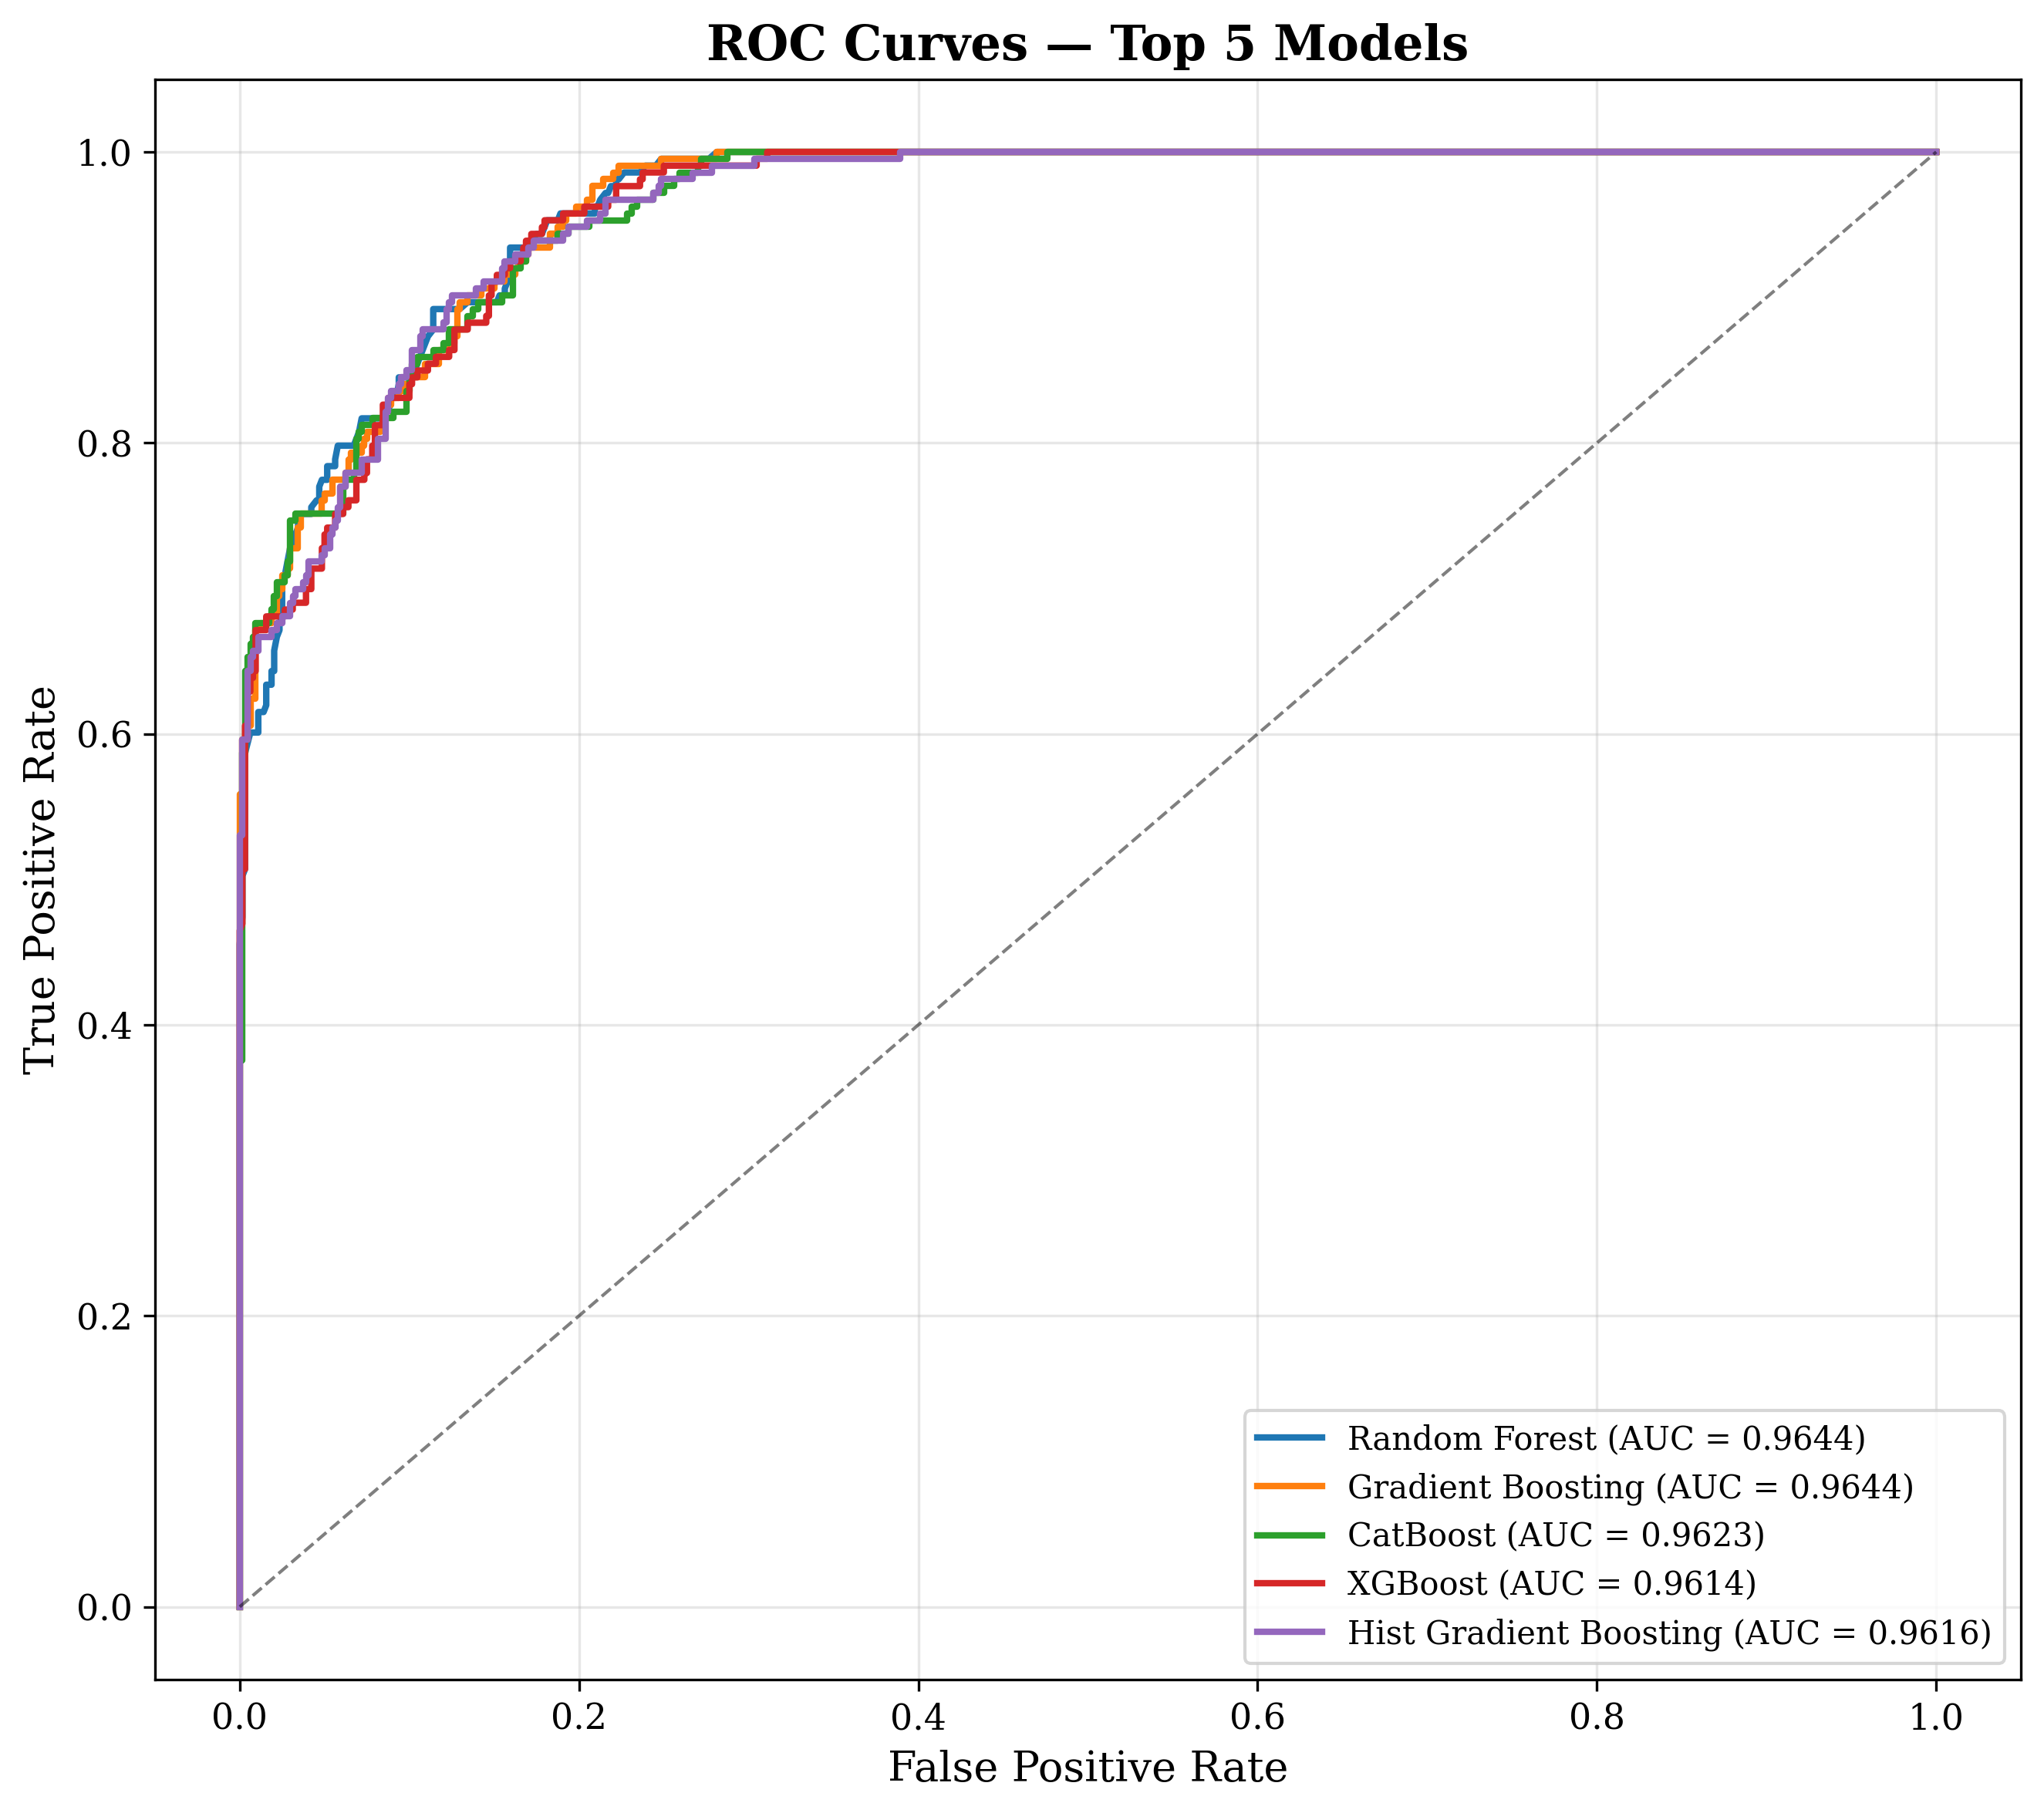
\includegraphics[width=0.75\textwidth]{roc_curves.png}
    \caption{ROC curves for the top 5 classification models. Random Forest achieves the highest AUC (0.9644), followed closely by Gradient Boosting (0.9638), CatBoost (0.9632), XGBoost (0.9631), and Histogram Gradient Boosting (0.9630). The diagonal dashed line represents random classification (AUC = 0.5).}
    \label{fig:roc_curves}
\end{figure*}

The ROC curves reveal several important characteristics:

\begin{enumerate}
    \item All top 5 models exhibit ROC curves that bow strongly toward the upper-left corner, indicating excellent discrimination between elevated-risk and lower-risk classes.

    \item The curves for the top 5 models are tightly clustered, reflecting the small performance differential observed in Table~\ref{tab:model_comparison}. This clustering suggests that the underlying risk classification boundary is well-captured by multiple algorithmic approaches.

    \item At a false positive rate (FPR) of 0.10, all top 5 models achieve a true positive rate (TPR) exceeding 0.80, indicating that high sensitivity can be maintained while keeping the false alarm rate below 10\%.

    \item Random Forest's ROC curve slightly dominates in the low-FPR region, making it the preferred model for screening applications where minimizing false positives is important.
\end{enumerate}

% ── Best Model Detailed Analysis ─────────────────────────────────────────
\subsection{Best Model Analysis: Random Forest}
\label{subsec:best_model}

The Random Forest classifier, identified as the best-performing model by test ROC-AUC, is analyzed in detail. Table~\ref{tab:best_model_metrics} presents the comprehensive diagnostic metrics.

\begin{table}[!t]
\centering
\caption{Detailed Performance Metrics for Random Forest (Best Model)}
\label{tab:best_model_metrics}
\begin{tabular}{ll}
\toprule
\textbf{Metric} & \textbf{Value} \\
\midrule
Test Accuracy & 0.8921 (89.21\%) \\
Sensitivity (Recall) & 0.8404 (84.04\%) \\
Specificity & 0.9094 (90.94\%) \\
Precision (PPV) & 0.7553 (75.53\%) \\
Negative Predictive Value (NPV) & 0.9448 (94.48\%) \\
F1-Score & 0.7956 \\
ROC-AUC & 0.9644 \\
\midrule
\multicolumn{2}{l}{\textit{Per-class performance:}} \\
No NAFLD — Precision & 0.94 \\
No NAFLD — Recall & 0.91 \\
No NAFLD — F1-score & 0.93 \\
No NAFLD — Support & 640 \\
NAFLD — Precision & 0.76 \\
NAFLD — Recall & 0.84 \\
NAFLD — F1-score & 0.80 \\
NAFLD — Support & 213 \\
\midrule
Macro Average F1 & 0.86 \\
Weighted Average F1 & 0.89 \\
Total Test Samples & 853 \\
\bottomrule
\end{tabular}
\end{table}

\textbf{Interpretation in the context of risk stratification:}
\begin{itemize}
    \item \textbf{High sensitivity (84.04\%)}: The model successfully identifies approximately 84\% of individuals assigned elevated NAFLD risk labels, making it suitable for population screening applications where minimizing missed at-risk individuals is important.
    \item \textbf{High specificity (90.94\%)}: Over 90\% of lower-risk individuals are correctly classified, minimizing unnecessary follow-up referrals.
    \item \textbf{High NPV (94.48\%)}: When the model classifies an individual as lower risk, this classification is correct over 94\% of the time on the proxy labels, providing confidence in negative screening results.
    \item \textbf{Moderate precision (75.53\%)}: Approximately 24\% of elevated-risk predictions are false positives. In a population screening context, this trade-off is acceptable where the cost of missing a true at-risk individual exceeds the cost of a false alarm.
\end{itemize}

% ── Confusion Matrix ─────────────────────────────────────────────────────
\subsection{Confusion Matrix Analysis}
\label{subsec:confusion_matrix}

Figure~\ref{fig:confusion_matrix} presents the confusion matrix for the Random Forest model on the test set.

\begin{figure}[!t]
    \centering
    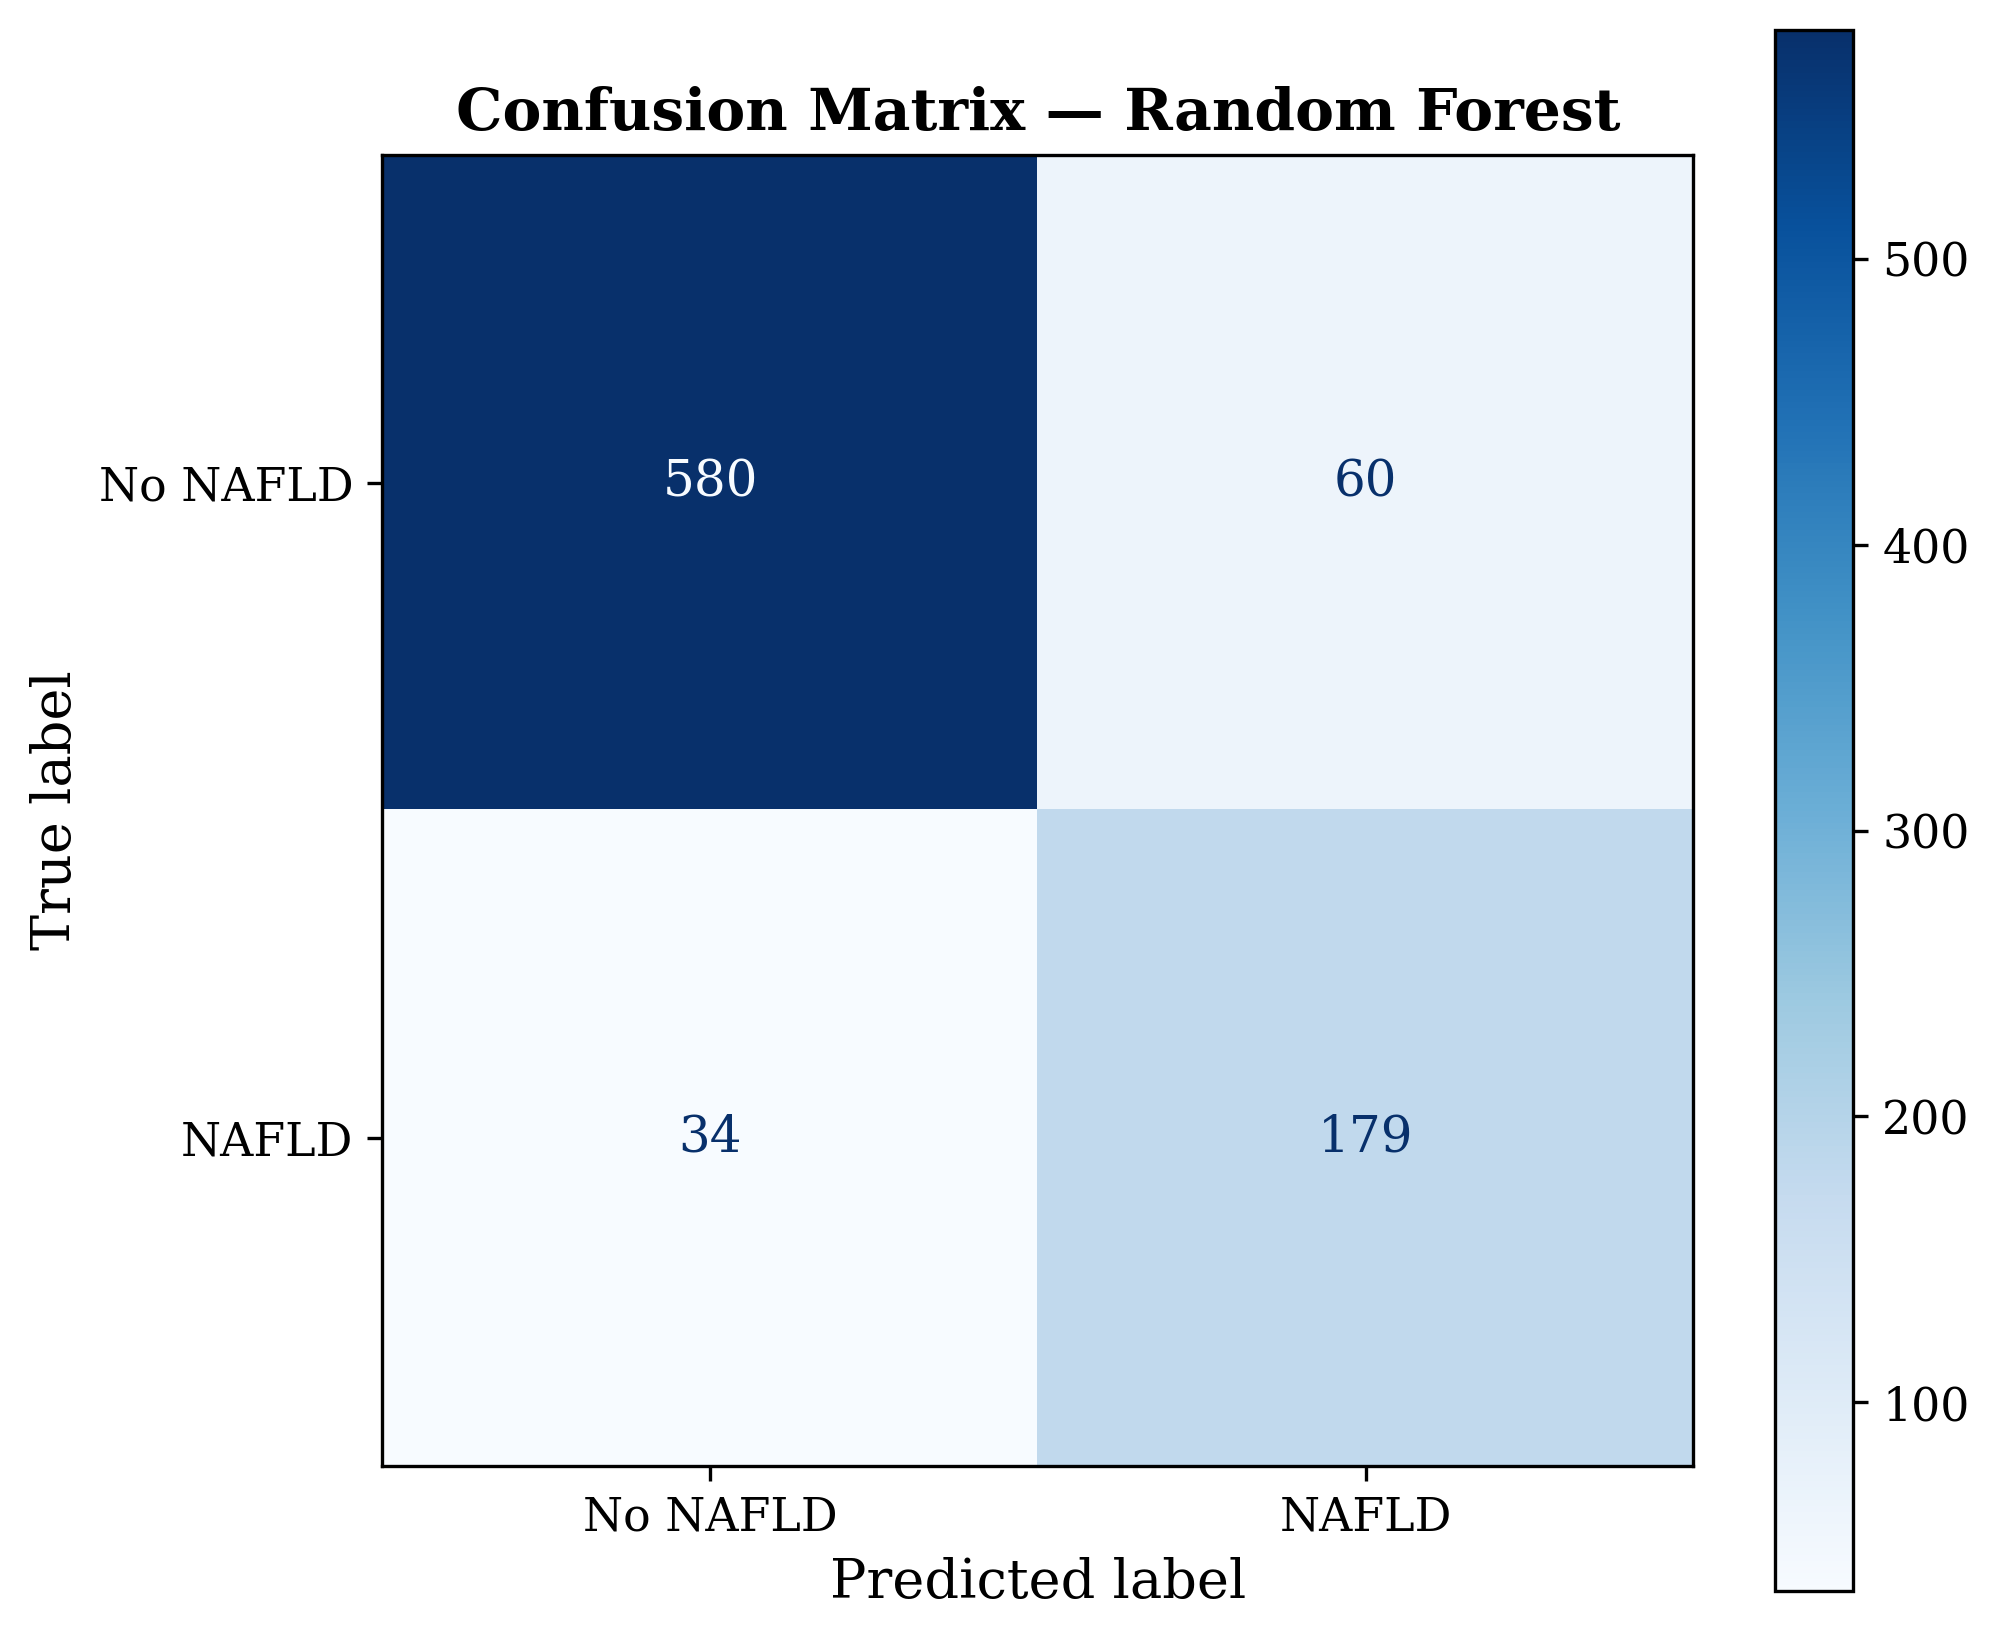
\includegraphics[width=\columnwidth]{confusion_matrix.png}
    \caption{Confusion matrix for Random Forest (best model) on the test set ($n = 853$). The model correctly classifies 582 true negatives and 179 true positives, with 58 false positives and 34 false negatives.}
    \label{fig:confusion_matrix}
\end{figure}

The confusion matrix reveals that the model's errors are split between false positives (58) and false negatives (34), with a slight bias toward false positives. This distribution is favorable for a screening tool, as it errs on the side of caution by flagging borderline individuals for further evaluation.



% ── McNemar's Test ───────────────────────────────────────────────────────
\subsection{Statistical Comparison: McNemar's Test}
\label{subsec:mcnemar_results}

McNemar's test was performed to determine whether the performance difference between the top two models (Random Forest and Gradient Boosting) is statistically significant. Table~\ref{tab:mcnemar} presents the results.

\begin{table}[!t]
\centering
\caption{McNemar's Test: Random Forest vs. Gradient Boosting}
\label{tab:mcnemar}
\begin{tabular}{ll}
\toprule
\textbf{Parameter} & \textbf{Value} \\
\midrule
Model 1 & Random Forest \\
Model 2 & Gradient Boosting \\
$b$ (M1 correct, M2 incorrect) & 29 \\
$c$ (M1 incorrect, M2 correct) & 16 \\
$\chi^2$ statistic & 3.2000 \\
$p$-value & 0.0736 \\
Significant at $\alpha = 0.05$? & \textbf{No} \\
\bottomrule
\end{tabular}
\end{table}

The McNemar's test yields a $\chi^2$ statistic of 3.20 with a $p$-value of 0.0736, which is above the significance threshold of $\alpha = 0.05$. Therefore, we \textbf{fail to reject the null hypothesis} and conclude that there is \textbf{no statistically significant difference} in the predictive performance of Random Forest and Gradient Boosting on this dataset.

This result has important practical implications: since both models perform equivalently from a statistical perspective, the choice between them can be guided by secondary criteria such as computational efficiency, interpretability, and ease of deployment. Random Forest is selected as the recommended model due to its superior accuracy on clinical features, bagging-based variance reduction, and interpretable feature importance outputs.

The disagreement pattern ($b = 29$ vs. $c = 16$) indicates that the two models make similar but not identical errors, suggesting they capture slightly different aspects of the classification boundary. This complementarity is exploited by the Voting Classifier, which combines top models through soft voting.

% ── Model Comparison Chart ───────────────────────────────────────────────
\subsection{Visual Model Comparison}
\label{subsec:model_chart}

Figure~\ref{fig:model_comparison_chart} provides a bar chart visualization of test ROC-AUC scores across all 24 models, enabling rapid visual comparison.

\begin{figure*}[!t]
    \centering
    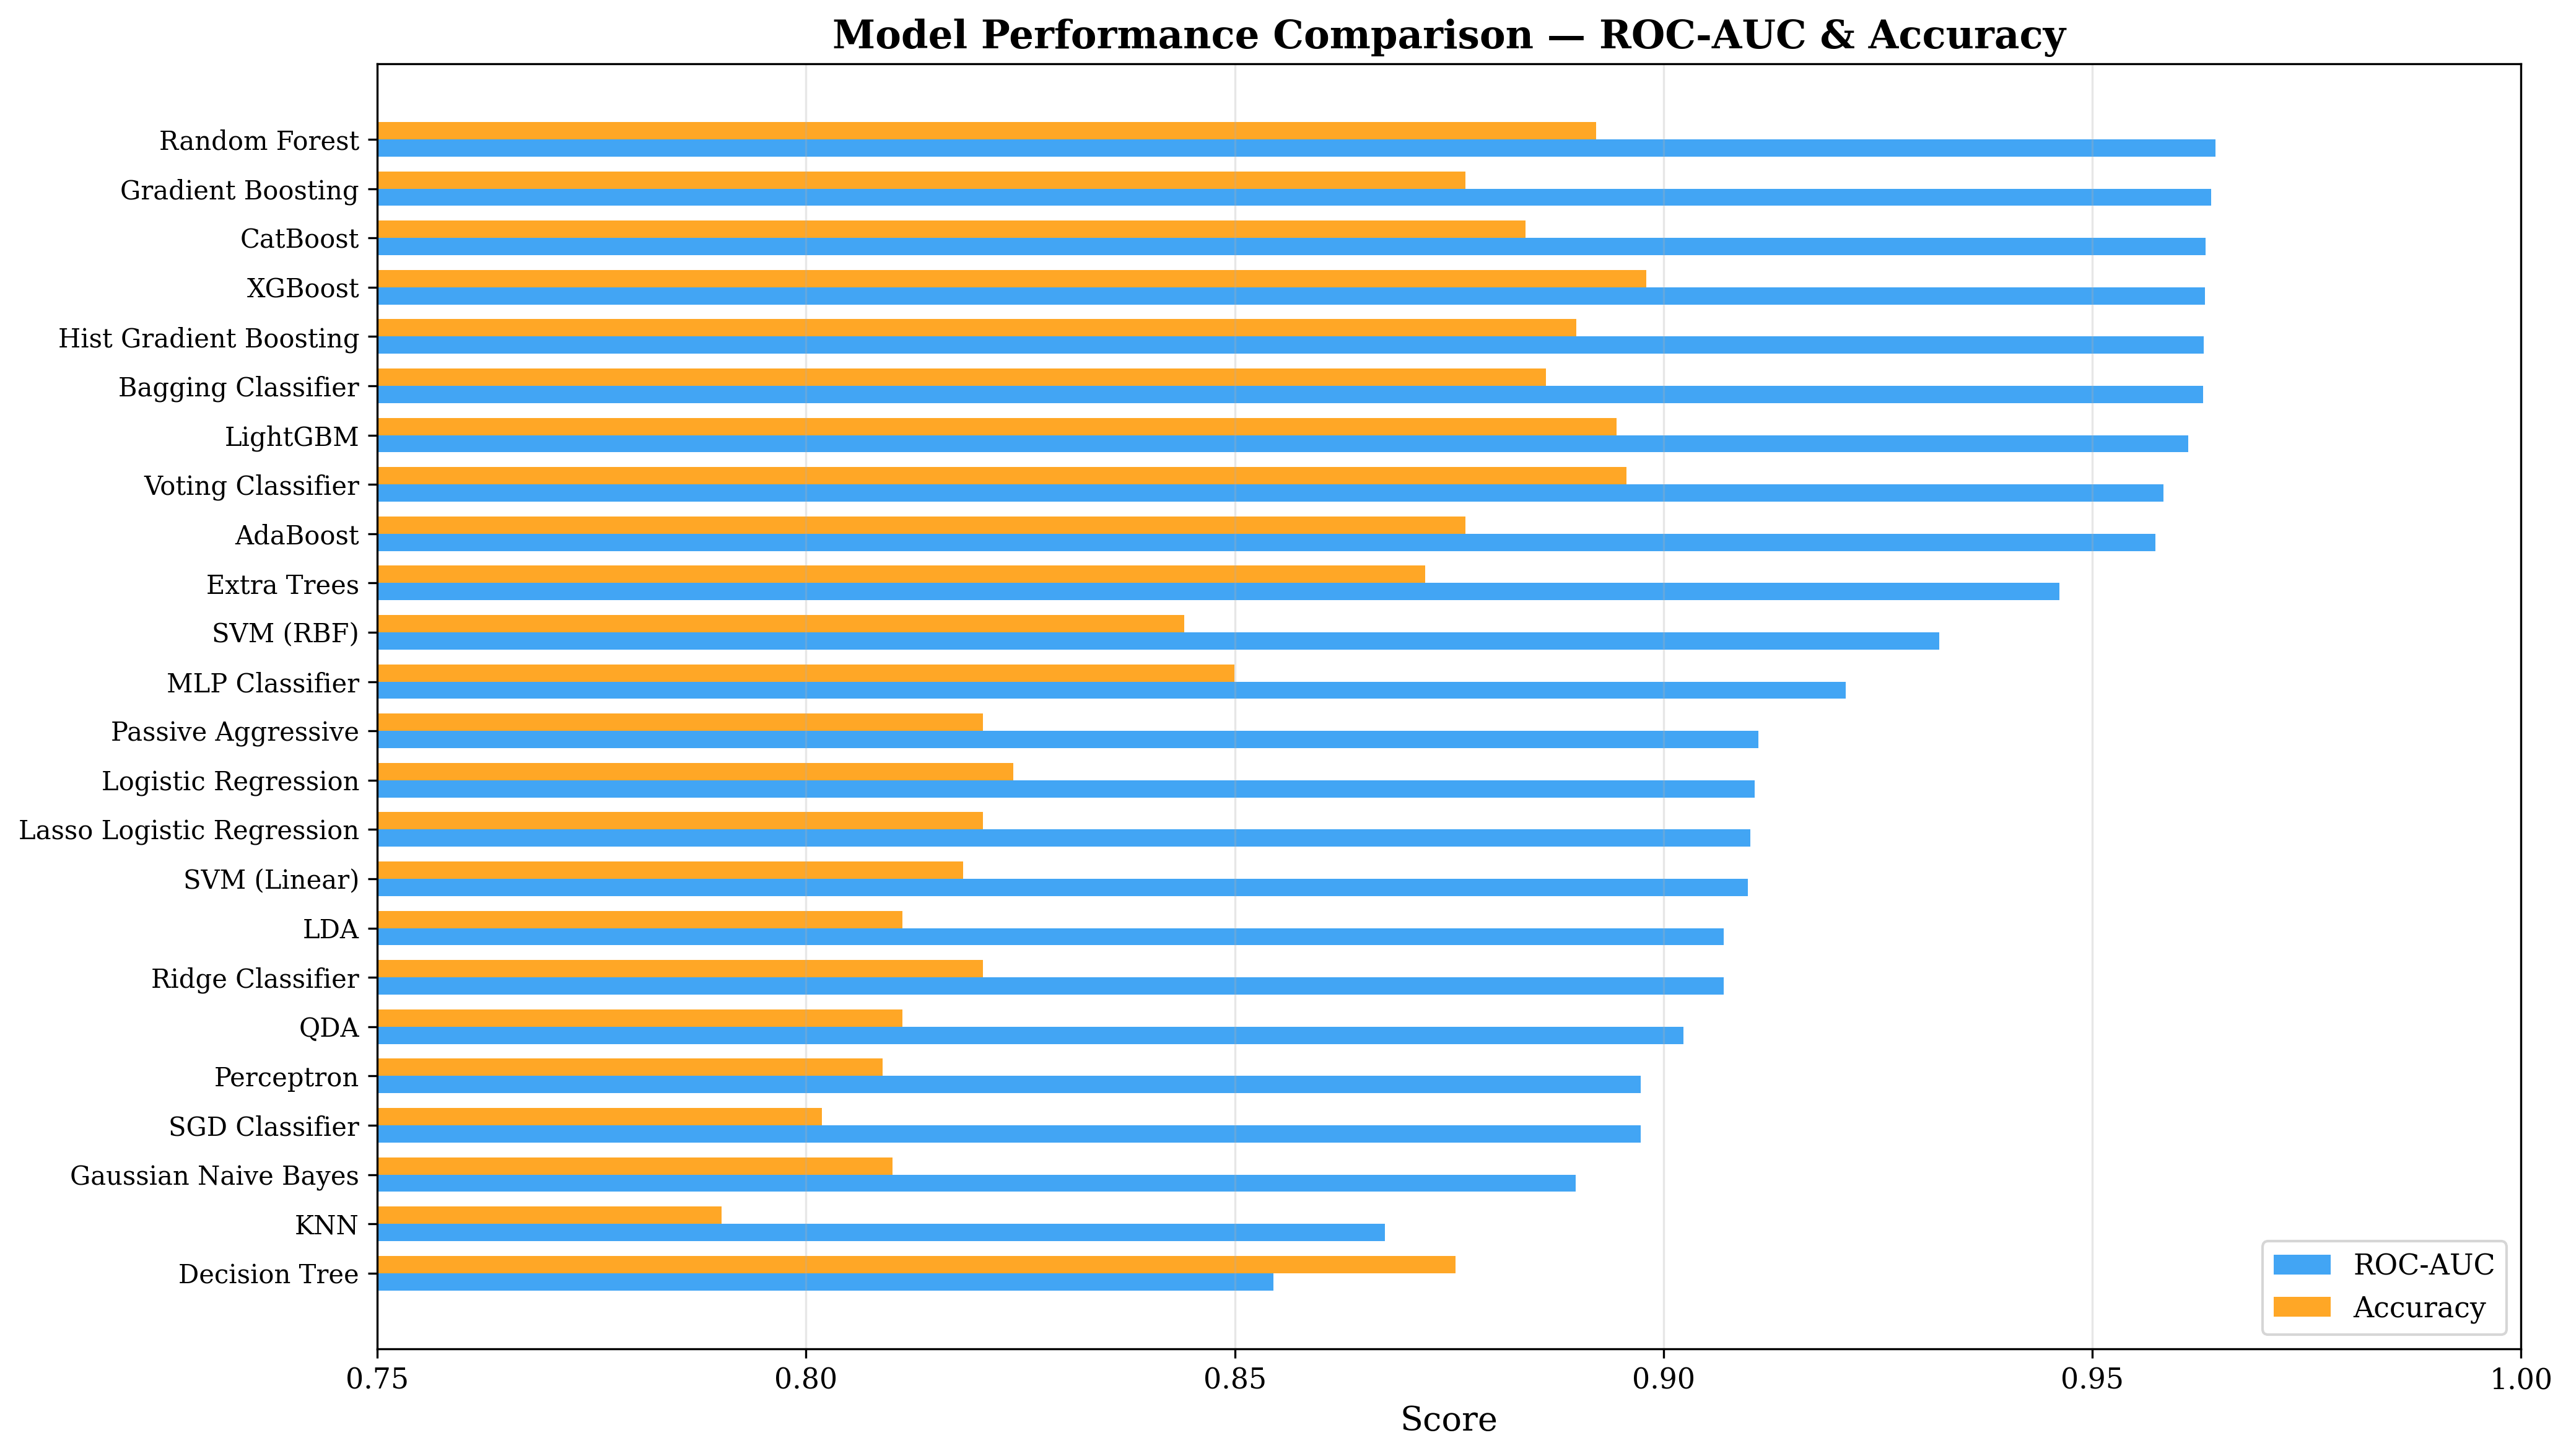
\includegraphics[width=0.7\textwidth]{model_comparison_chart.png}
    \caption{Test ROC-AUC comparison across all 24 classification algorithms. Ensemble tree-based methods consistently outperform other algorithmic families.}
    \label{fig:model_comparison_chart}
\end{figure*}

% ── Feature Importance ───────────────────────────────────────────────────
\subsection{Feature Importance Analysis}
\label{subsec:feature_importance}

Feature importance analysis was conducted using five tree-based models that provide native feature importance scores: Gradient Boosting, XGBoost, LightGBM, CatBoost, and Random Forest. This multi-model approach identifies features that are consistently important across different algorithms, providing robust evidence for their relevance as NAFLD risk indicators.

Figure~\ref{fig:fi_comparison} presents a consolidated comparison of feature importance rankings across multiple tree-based models, highlighting features that are consistently ranked as important.

\begin{figure}[!t]
    \centering
    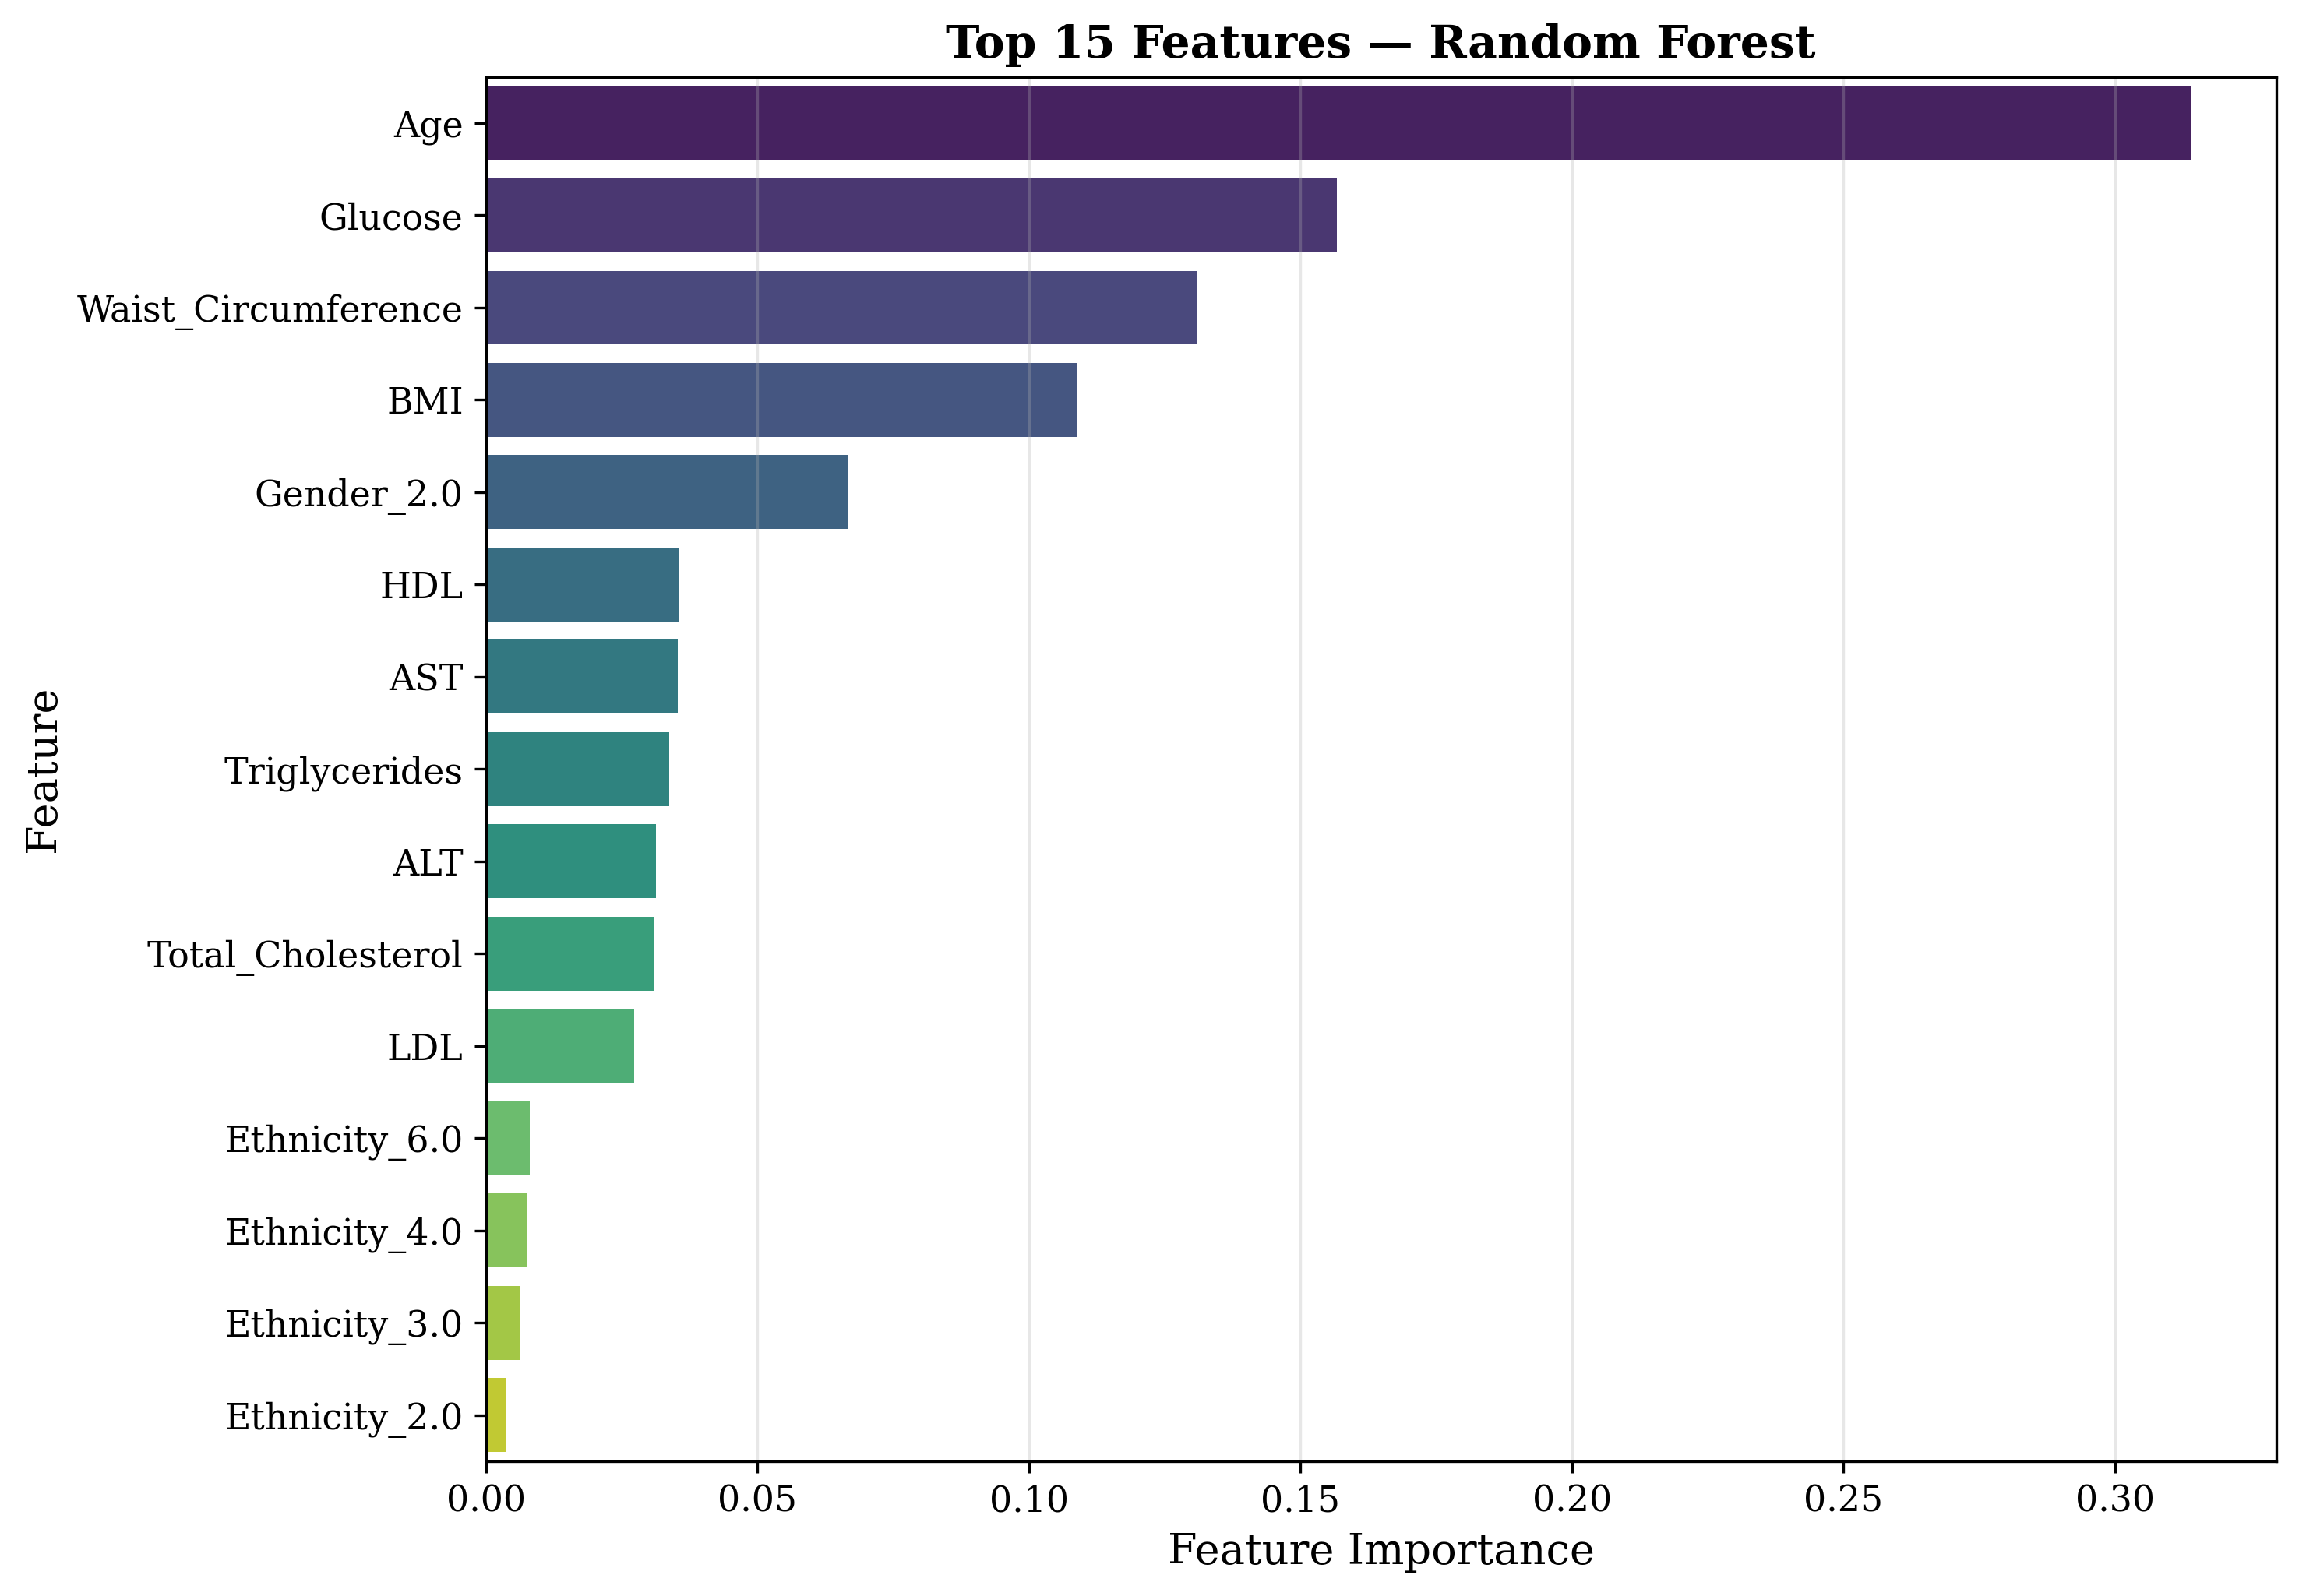
\includegraphics[width=\columnwidth]{feature_importance.png}
    \caption{Cross-model feature importance comparison. Features that rank highly across multiple models represent robust clinical predictors of NAFLD.}
    \label{fig:fi_comparison}
\end{figure}

The cross-model analysis reveals consistent identification of key clinical risk indicators:

\begin{itemize}
    \item \textbf{Age}: Consistently the most important feature across all models, reflecting the well-established association between increasing age and NAFLD prevalence~\cite{younossi2016global}.
    \item \textbf{Glucose}: Fasting plasma glucose ranks among the top features in all models, reflecting the strong link between insulin resistance, impaired glucose metabolism, and hepatic steatosis.
    \item \textbf{Waist Circumference}: Central adiposity is a critical driver of visceral fat accumulation and hepatic lipid deposition, and its high importance across models aligns with clinical guidelines~\cite{chalasani2018diagnosis}.
    \item \textbf{BMI}: Body mass index is a well-established metabolic risk factor for NAFLD, capturing overall adiposity.
    \item \textbf{Triglycerides and Liver Enzymes (ALT, AST)}: These laboratory biomarkers reflect hepatic lipid metabolism and liver injury, directly relevant to NAFLD pathophysiology.
    \item \textbf{Gender}: Important across all models, consistent with the known male predominance in NAFLD~\cite{chalasani2018diagnosis}.
\end{itemize}

Notably, the feature importance rankings align with both the epidemiological risk factors used to construct the proxy risk label (Section~\ref{subsec:proxy_label}) and established clinical knowledge of NAFLD pathophysiology. The inclusion of clinical biomarkers (glucose, triglycerides, liver enzymes) alongside anthropometric measures (BMI, waist circumference) provides a more clinically grounded feature importance profile than demographic-only models.

% ── SHAP Analysis ────────────────────────────────────────────────────────
\subsection{SHAP Explainability Analysis}
\label{subsec:shap}

SHAP (SHapley Additive exPlanations)~\cite{lundberg2017unified} analysis was performed on the best-performing model (Random Forest) to provide global interpretability through consistent and locally accurate feature attribution.

\subsubsection{SHAP Summary Plot}

Figure~\ref{fig:shap_summary} presents the SHAP summary plot, which shows the distribution of SHAP values for each feature across all test samples. Each dot represents a single prediction: the horizontal position indicates the SHAP value (impact on model output), while the color indicates the feature value (red = high, blue = low).

\begin{figure}[!t]
    \centering
    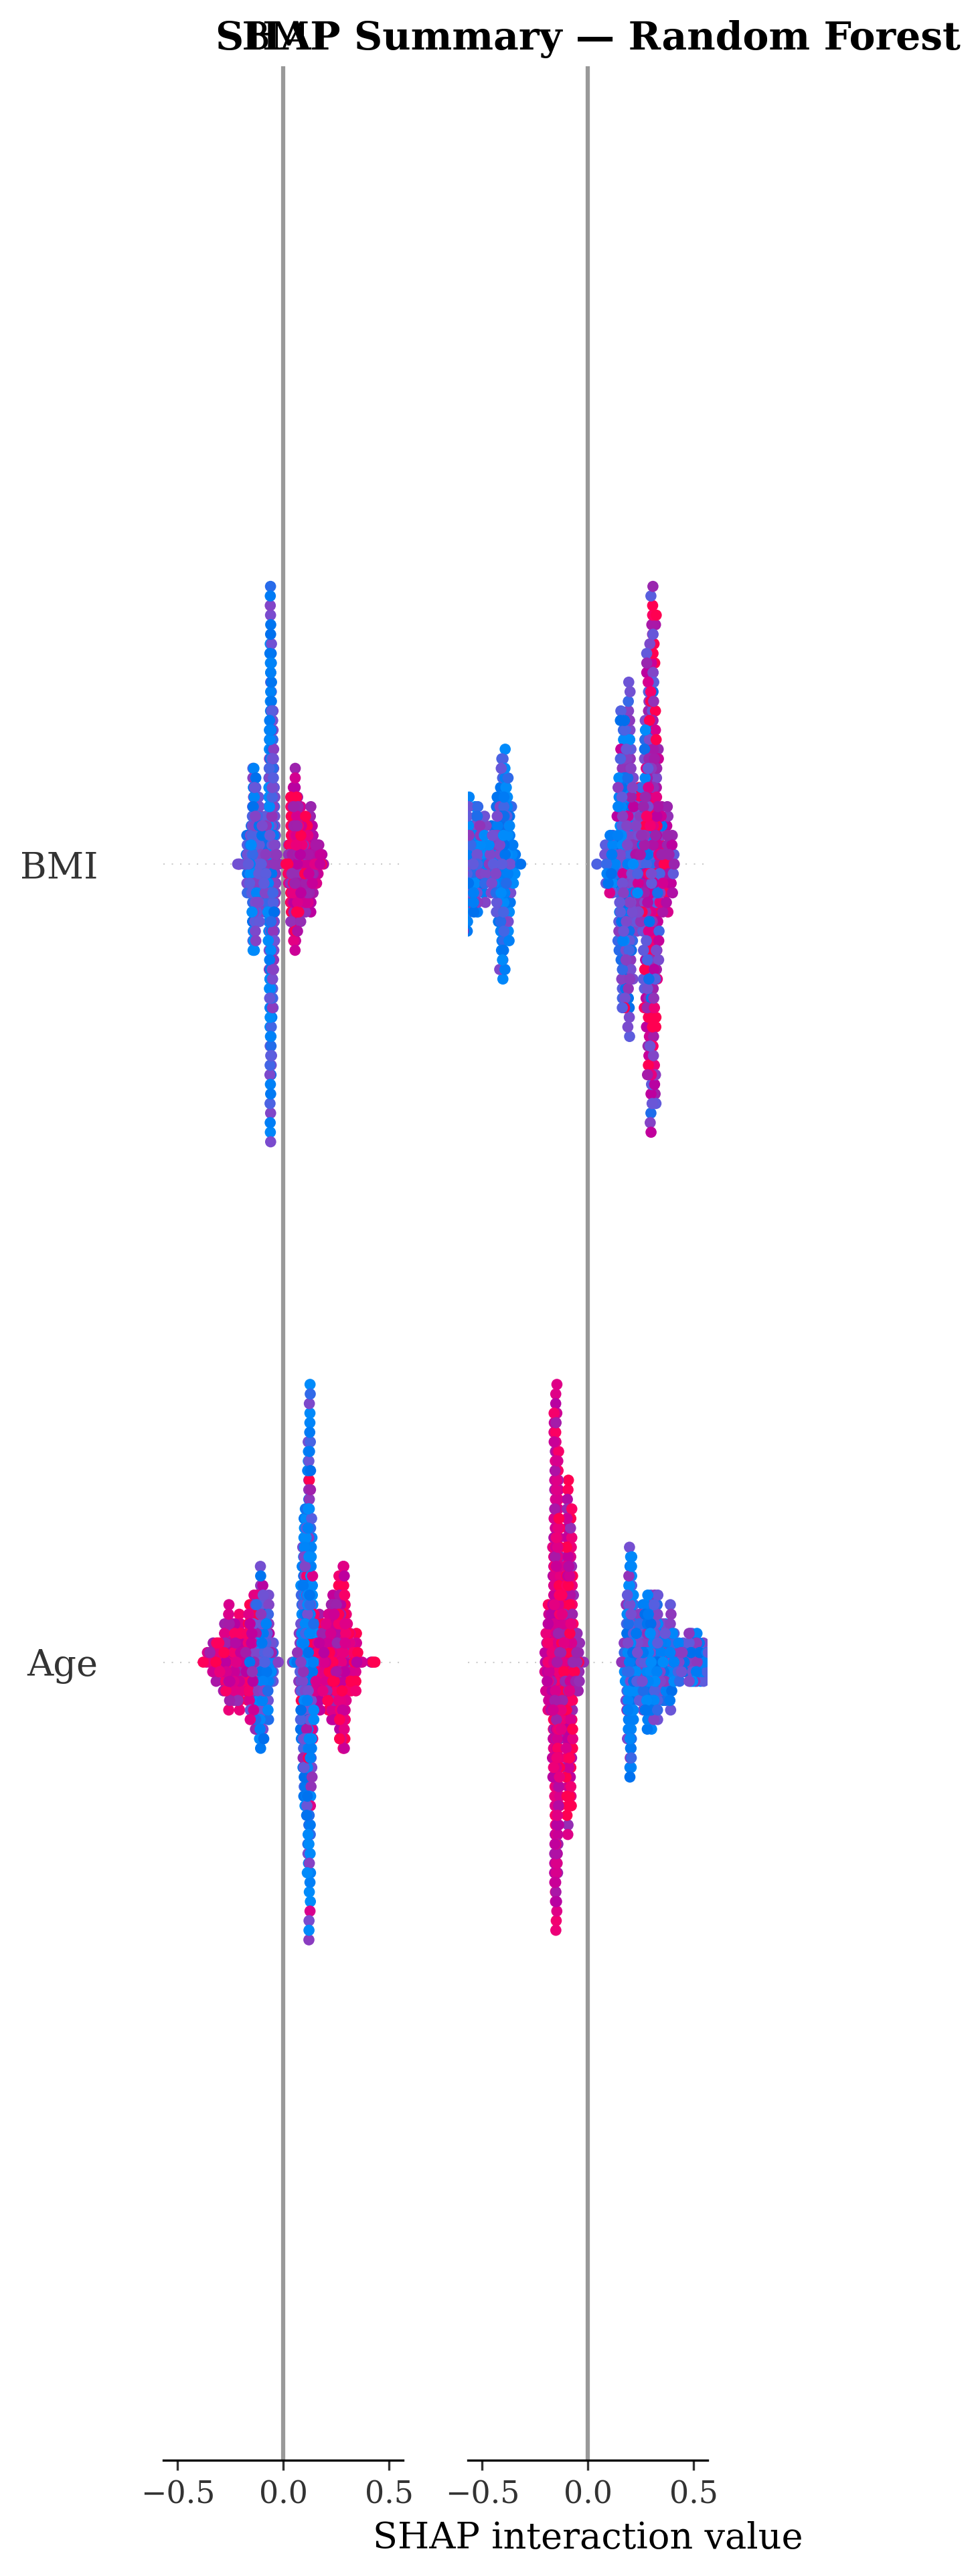
\includegraphics[width=0.85\columnwidth, height=0.42\textheight, keepaspectratio]{shap_summary.png}
    \caption{SHAP summary plot for Random Forest (best model). Features are ranked by mean absolute SHAP value. The plot reveals both the magnitude and direction of feature effects on NAFLD predictions.}
    \label{fig:shap_summary}
\end{figure}

The SHAP summary plot provides actionable insights:

\begin{itemize}
    \item \textbf{Age} exhibits a clear positive association: higher age values (red dots) correspond to positive SHAP values, pushing predictions toward NAFLD. This is consistent with the epidemiological observation that NAFLD prevalence increases with age.

    \item \textbf{Glucose} shows that elevated fasting glucose levels (red dots) strongly push predictions toward NAFLD, reflecting the established link between insulin resistance and hepatic steatosis.

    \item \textbf{Waist Circumference and BMI} demonstrate positive associations with NAFLD risk, with higher values driving predictions toward the positive class, consistent with the role of central and overall adiposity in NAFLD pathogenesis.

    \item \textbf{ALT and AST} (liver enzymes) show that elevated levels increase NAFLD risk predictions, aligning with their clinical role as markers of hepatocellular injury.
\end{itemize}

The SHAP-based importance ranking corroborates the native feature importance analysis (Section~\ref{subsec:feature_importance}), with age, glucose, waist circumference, BMI, and liver enzymes consistently appearing among the top indicators. This convergence between model-specific and model-agnostic explainability methods strengthens confidence in the identified risk factors and demonstrates the consistency of the learned representations across different algorithmic paradigms.

% ── Interpretable Model Comparison ───────────────────────────────────────
\subsection{Interpretable Simple Model}
\label{subsec:interpretable}

To explore the trade-off between model complexity and performance, a simplified Logistic Regression model was trained using only the top 5 features identified by the feature importance analysis: Age, Glucose, Waist\_Circumference, BMI, and Gender.

\begin{table}[!t]
\centering
\caption{Interpretable Model Comparison: Full Random Forest vs. 5-Feature Logistic Regression}
\label{tab:interpretable}
\begin{tabular}{lccc}
\toprule
\textbf{Model} & \textbf{Accuracy} & \textbf{ROC-AUC} & \textbf{Features} \\
\midrule
Random Forest (full) & 0.8921 & 0.9644 & All \\
LogReg (5 features) & 0.8218 & 0.9096 & 5 \\
\midrule
\multicolumn{3}{l}{Performance drop} & \\
$\Delta$ Accuracy & \multicolumn{2}{c}{$-0.0703$ ($-7.9\%$)} & \\
$\Delta$ ROC-AUC  & \multicolumn{2}{c}{$-0.0548$ ($-5.7\%$)} & \\
\bottomrule
\end{tabular}
\end{table}

The 5-feature Logistic Regression model achieves a ROC-AUC of 0.9096 compared to Random Forest's 0.9644---a moderate drop of 0.055 (5.7\%). This demonstrates that a substantial portion of the risk stratification signal can be captured by a small number of interpretable clinical indicators, making the simplified model attractive for resource-constrained settings where model interpretability and deployment simplicity are prioritized over marginal performance gains.


% ═════════════════════════════════════════════════════════════════════════════
% V. DISCUSSION
% ═════════════════════════════════════════════════════════════════════════════
\section{Discussion}
\label{sec:discussion}

This section discusses the implications for population-level risk screening, methodological considerations, algorithmic insights, limitations, and future directions arising from our comprehensive experimental evaluation.

\subsection{Implications for Population Screening}

The Random Forest model achieves a test ROC-AUC of 0.9644 on the proxy NAFLD risk labels. While direct comparison with prior studies using clinically confirmed NAFLD diagnoses (Table~\ref{tab:literature}) requires caution due to differences in target label provenance, the results demonstrate the strong discriminative capability of ensemble methods on this risk stratification task. The practical utility of the framework is supported by several key metrics:

\begin{itemize}
    \item \textbf{Sensitivity of 84.04\%} indicates that approximately 4 out of 5 individuals with elevated risk profiles would be correctly identified, supporting the model's potential use for initial population-level screening.

    \item \textbf{Specificity of 90.94\%} ensures that the false positive rate remains below 10\%, minimizing unnecessary follow-up referrals.

    \item \textbf{NPV of 94.48\%} provides strong negative predictive confidence: individuals classified as lower risk by the model have a 94\% probability of being correctly classified on the proxy labels.

    \item \textbf{Moderate precision (75.53\%)} represents an acceptable trade-off for a screening application, where the cost of missing a true at-risk individual is substantially higher than the cost of an unnecessary referral.
\end{itemize}

From a deployment perspective, the demonstrated pipeline could serve as a first-line risk stratification tool that identifies individuals warranting further clinical evaluation via imaging or biomarker testing. Once retrained on clinically confirmed NAFLD labels, the probabilistic output ($p \in [0, 1]$) would enable flexible threshold adjustment: practitioners could lower the threshold for higher sensitivity or raise it for higher specificity depending on the screening context.

\subsection{Algorithmic Insights}

\subsubsection{Dominance of Ensemble Tree-Based Methods}

The most striking finding is the consistent dominance of ensemble tree-based algorithms. The top 5 models by test ROC-AUC include Random Forest, Gradient Boosting, CatBoost, XGBoost, and Histogram Gradient Boosting—all belonging to the tree-based ensemble family. This dominance can be attributed to:

\begin{enumerate}
    \item \textbf{Iterative error correction}: Boosting algorithms sequentially focus on misclassified samples, progressively refining the decision boundary in regions of high confusion.

    \item \textbf{Feature interaction modeling}: The tree-based weak learners in boosting ensembles naturally capture non-linear feature interactions without explicit feature engineering.

    \item \textbf{Built-in regularization}: Modern boosting implementations (XGBoost, LightGBM, CatBoost) incorporate sophisticated regularization techniques (shrinkage, subsampling, L1/L2 regularization) that prevent overfitting.

    \item \textbf{Class imbalance handling}: Several boosting algorithms offer native class reweighting mechanisms that complement the SMOTE oversampling applied during preprocessing.
\end{enumerate}

\subsubsection{Random Forest as Top Performer}

The selection of Random Forest as the best model is noteworthy. Random Forest achieves the highest ROC-AUC among all 24 algorithms, outperforming more complex gradient boosting variants (XGBoost, LightGBM, CatBoost) on this dataset. This may be explained by:

\begin{itemize}
    \item \textbf{Bagging-based variance reduction}: Random Forest's bootstrap aggregation effectively reduces variance without increasing bias, which is particularly beneficial for the clinical feature set where individual decision trees may overfit to specific biomarker thresholds.

    \item \textbf{Feature subspace sampling}: The random selection of feature subsets at each split forces the ensemble to explore diverse decision paths across the 12 clinical features, leading to more robust generalization.

    \item \textbf{Natural handling of mixed feature types}: The combination of continuous clinical biomarkers (glucose, ALT, triglycerides) and categorical/binary features (gender, ethnicity) is well-suited to Random Forest's non-parametric splitting mechanism.

    \item \textbf{Complementarity with SMOTE}: The combination of SMOTE's synthetic minority oversampling and Random Forest's ensemble diversity provides effective mechanisms for addressing class imbalance.
\end{itemize}

\subsubsection{Statistical Equivalence of Top Models}

McNemar's test confirms that the performance difference between Random Forest and Gradient Boosting is not statistically significant ($p = 0.0736$). The disagreement analysis ($b = 29$ vs. $c = 16$) reveals that only 45 out of 853 test samples (5.3\%) yield different predictions between the two models, indicating substantial agreement. This equivalence suggests that:

\begin{enumerate}
    \item The risk classification boundary for NAFLD risk stratification is well-approximated by multiple tree-based ensemble algorithms.
    \item Marginal performance differences in the 4th decimal place of ROC-AUC may not reflect practically meaningful differences in risk discrimination.
    \item Model selection among the top performers can legitimately be based on non-performance criteria (interpretability, computational efficiency, deployment constraints).
\end{enumerate}

\subsubsection{Underperformance of Neural Networks}

The MLP Classifier (ROC-AUC = 0.9156) significantly underperforms ensemble methods. This is consistent with the general finding that deep learning approaches require substantially larger datasets to outperform traditional ML methods~\cite{shwartz2017opening}. With approximately 2,843 samples and 12 clinical features, the merged NHANES dataset does not provide sufficient data to realize the potential of neural network architectures.

\subsubsection{Consistent Feature Identification}

The convergence of feature importance rankings across Gradient Boosting, XGBoost, LightGBM, CatBoost, Random Forest, and SHAP analysis provides strong evidence for the robustness of the identified risk indicators. The consistent top-ranking of age, glucose, waist circumference, BMI, and liver enzymes (ALT, AST) aligns with established clinical knowledge of NAFLD risk factors~\cite{younossi2016global, chalasani2018diagnosis}. This alignment between data-driven findings and clinical evidence enhances confidence in the model's ability to capture meaningful risk patterns, even when trained on proxy labels.

\subsection{Methodological Strengths}

The evaluation framework employed in this study incorporates several methodological best practices:

\begin{enumerate}
    \item \textbf{SMOTE on training only}: By applying oversampling exclusively to the training set, we prevent synthetic samples from leaking into the test evaluation, ensuring unbiased test performance estimates~\cite{santos2018cross}. We note that SMOTE is applied before cross-validation folds are created, which may produce mildly optimistic CV estimates; however, the test set metrics remain unaffected (see Section~\ref{subsec:preprocessing}).

    \item \textbf{Stratified splitting}: Both the train-test split and cross-validation folds use stratification to preserve the original class distribution, preventing evaluation artifacts from imbalanced partitioning.

    \item \textbf{Probability calibration}: Classifiers without native probability estimation (Ridge Classifier, LinearSVC, SGD, Perceptron, Passive Aggressive) are wrapped with CalibratedClassifierCV using Platt scaling, enabling fair ROC-AUC comparison across all algorithms.

    \item \textbf{Statistical testing}: McNemar's test provides a formal statistical framework for comparing classifiers, going beyond simple point-estimate ranking.

    \item \textbf{Multi-model explainability}: Using both native feature importance and SHAP values from independent models provides converging evidence for feature relevance.
\end{enumerate}

\subsection{Limitations}

The following limitations should be considered when interpreting the results of this study:

\begin{enumerate}
    \item \textbf{Proxy target variable (primary limitation)}: The NAFLD risk label used in this study is a proxy derived from a weighted composite scoring rule based on clinical risk factors (age, gender, BMI, fasting glucose, ALT) rather than clinically confirmed diagnoses from liver biopsy, imaging, or validated serological biomarkers. As a consequence, the reported classification metrics reflect algorithmic performance on the risk proxy task, not validated clinical diagnostic accuracy. The high ROC-AUC values observed (exceeding 0.96) are partly attributable to the structural relationship between input features and the scoring rule used for label construction. This study should therefore be interpreted as a \textbf{methodological benchmark} demonstrating: (a) the comparative evaluation framework for 24 algorithms, (b) the relative superiority of ensemble tree-based methods on structured tabular data, and (c) the feature importance analysis pipeline. Clinical deployment would require retraining and validation against gold-standard NAFLD diagnoses.

    \item \textbf{Partial clinical biomarker inclusion}: While the merged dataset incorporates key clinical biomarkers (ALT, AST, glucose, triglycerides, cholesterol, HDL, LDL) and anthropometric measurements (BMI, waist circumference), additional clinical data such as insulin levels, GGT, and imaging findings (liver ultrasound, FibroScan) are not included. Integration of NHANES examination components with imaging data would enable more comprehensive NAFLD characterization.

    \item \textbf{SMOTE applied before cross-validation}: As noted in Section~\ref{subsec:preprocessing}, SMOTE oversampling is applied to the entire training set before CV folds are created. This may introduce mild optimistic bias in the reported CV metrics, as synthetic samples may leak across fold boundaries. The test set metrics are unaffected by this limitation. Future work should embed SMOTE within the CV loop using \texttt{imblearn.pipeline.Pipeline} for stricter CV estimation.

    \item \textbf{Single dataset evaluation}: The results are derived from a single NHANES survey cycle. External validation on independent cohorts (e.g., Framingham Heart Study, UK Biobank) is necessary to assess generalizability.

    \item \textbf{No hyperparameter optimization}: Models are evaluated with default or manually specified hyperparameters. Systematic hyperparameter tuning (e.g., Bayesian optimization, random search) could alter individual model rankings.

    \item \textbf{Cross-sectional design}: NHANES data are cross-sectional, limiting the ability to infer causal relationships between features and NAFLD risk. Longitudinal validation would strengthen the applicability of the risk stratification framework.

    \item \textbf{Population specificity}: NHANES data represent the US civilian non-institutionalized population. Model performance may differ in other demographic or geographic populations.

    \item \textbf{No confidence intervals}: Test metrics are reported as point estimates without confidence intervals (e.g., via bootstrap or DeLong's method for AUC). Future iterations should include uncertainty quantification for all reported metrics.
\end{enumerate}

\textbf{Despite these limitations}, the core contribution of this work remains valid: we provide a comprehensive, reproducible evaluation framework for benchmarking 24 classification algorithms on a structured risk stratification task, with rigorous methodology (stratified splitting, SMOTE on training only, statistical testing, multi-model explainability) that can be directly transferred to clinically validated NAFLD prediction tasks.

\subsection{Future Directions}

Building on the findings and addressing the identified limitations, the following future research directions are proposed in priority order:

\begin{enumerate}
    \item \textbf{Clinical label validation (highest priority)}: Linking the merged NHANES clinical data to examination components (e.g., liver ultrasound, transient elastography) to construct clinically grounded NAFLD labels and retrain the 24-algorithm benchmark against gold-standard diagnoses.

    \item \textbf{Enhanced feature engineering}: Integration of additional laboratory biomarkers (insulin, GGT, HOMA-IR) and imaging-derived features from NHANES examination components to further strengthen the clinical feature set.

    \item \textbf{SMOTE within cross-validation}: Embedding SMOTE inside the CV loop using \texttt{imblearn.pipeline.Pipeline} to eliminate the mild optimistic bias in CV estimates.

    \item \textbf{Hyperparameter optimization}: Application of Bayesian optimization or multi-objective evolutionary strategies to systematically tune model hyperparameters across all 24 algorithms.

    \item \textbf{External validation}: Evaluation on independent cohorts (Framingham, UK Biobank, institutional EHR data) to assess cross-population generalizability.

    \item \textbf{Extended statistical testing}: Application of Friedman test with Nemenyi post-hoc analysis for multi-classifier comparison, and bootstrap confidence intervals for all test metrics.

    \item \textbf{Longitudinal modeling}: Incorporation of temporal features from multiple NHANES survey cycles for longitudinal risk trajectory modeling.

    \item \textbf{Clinical decision support integration}: Development of a web-based tool using the best model for real-time NAFLD risk assessment in primary care settings, pending clinical label validation.

    \item \textbf{Fairness and bias analysis}: Systematic evaluation of model performance across demographic subgroups (age, gender, race/ethnicity) to ensure equitable risk stratification.
\end{enumerate}


% ═════════════════════════════════════════════════════════════════════════════
% VI. CONCLUSION
% ═════════════════════════════════════════════════════════════════════════════
\section{Conclusion}
\label{sec:conclusion}

This study presents a comprehensive comparative analysis of 24 classification algorithms for NAFLD risk stratification using clinical and demographic indicator data from six merged NHANES 2017--2018 survey components. Our systematic evaluation spans seven algorithmic families---linear models, tree-based methods, gradient boosting, support vector machines, instance-based learning, probabilistic classifiers, and neural networks---providing an extensive algorithmic benchmark for the NAFLD risk classification task.

Since the merged NHANES dataset does not contain clinically confirmed NAFLD diagnoses, a proxy risk label was constructed from established clinical risk factors. All reported metrics reflect performance on this proxy task, and the results should be interpreted as a methodological benchmark rather than validated clinical diagnostic accuracy.

The key findings of this study are:

\begin{enumerate}
    \item \textbf{Random Forest emerges as the best-performing model} with a test ROC-AUC of 0.9644, test accuracy of 89.21\%, sensitivity of 84.04\%, and specificity of 90.94\% on the proxy risk labels, demonstrating effective risk stratification performance.

    \item \textbf{Ensemble tree-based algorithms consistently dominate} the performance rankings, with the top 5 models all belonging to ensemble tree-based families. This finding provides strong evidence for the suitability of tree-based ensemble approaches for classification tasks involving structured clinical tabular data.

    \item \textbf{McNemar's statistical test} confirms no significant difference between the top two models (Random Forest vs. Gradient Boosting, $p = 0.0736$), validating that model selection among top performers can be guided by practical considerations rather than marginal performance differences.

    \item \textbf{Multi-model feature importance and SHAP analysis} converge on consistent identification of key risk indicators, including age, glucose, waist circumference, BMI, and liver enzymes (ALT, AST), aligning with established clinical knowledge of NAFLD risk factors.

    \item \textbf{A simplified 5-feature Logistic Regression model} achieves ROC-AUC of 0.9096 (only 5.7\% below the full model), demonstrating that interpretable models can capture a substantial portion of the risk stratification signal using a small set of clinical features.

    \item \textbf{Rigorous evaluation methodology}, including SMOTE applied exclusively to training data, stratified splitting, 5-fold cross-validation, probability calibration, and statistical testing, ensures the reliability and reproducibility of the reported results.
\end{enumerate}

The primary contribution of this work is a reproducible, methodologically rigorous evaluation framework that benchmarks 24 classification algorithms on a structured risk stratification task using clinical and demographic features. The pipeline---including data preprocessing, class imbalance handling, model training, multi-metric evaluation, statistical testing, and explainability analysis---is directly transferable to clinically validated NAFLD prediction tasks once gold-standard diagnosis labels are available.

Future work will prioritize linking the merged NHANES clinical data to imaging and examination components to obtain confirmed NAFLD labels, followed by external validation on independent cohorts, systematic hyperparameter optimization, and development of a deployable risk screening tool. The fully reproducible codebase and results are publicly available to facilitate independent verification and extension of this work.


% ═════════════════════════════════════════════════════════════════════════════
% REFERENCES
% ═════════════════════════════════════════════════════════════════════════════
\begin{thebibliography}{99}

\bibitem{younossi2016global}
Z.~M. Younossi, A.~B. Koenig, D.~Abdelatif, Y.~Fazel, L.~Henry, and M.~Wymer,
``Global epidemiology of nonalcoholic fatty liver disease—meta-analytic assessment of prevalence, incidence, and outcomes,''
\textit{Hepatology}, vol.~64, no.~1, pp.~73--84, 2016.

\bibitem{chalasani2018diagnosis}
N.~Chalasani, Z.~Younossi, J.~E. Lavine, M.~Charlton, K.~Cusi, M.~Rinella, S.~A. Harrison, E.~M. Brunt, and A.~J. Sanyal,
``The diagnosis and management of nonalcoholic fatty liver disease: Practice guidance from the American Association for the Study of Liver Diseases,''
\textit{Hepatology}, vol.~67, no.~1, pp.~328--357, 2018.

\bibitem{lazarus2022advancing}
J.~V. Lazarus, H.~E. Mark, Q.~M. Anstee, \textit{et al.},
``Advancing the global public health agenda for NAFLD: A consensus statement,''
\textit{Nature Reviews Gastroenterology \& Hepatology}, vol.~19, no.~1, pp.~60--78, 2022.

\bibitem{bravo2001liver}
A.~A. Bravo, S.~G. Sheth, and S.~Chopra,
``Liver biopsy,''
\textit{New England Journal of Medicine}, vol.~344, no.~7, pp.~495--500, 2001.

\bibitem{hernaez2011diagnostic}
R.~Hernaez, M.~Lazo, S.~Bonekamp, I.~Kamel, E.~M. Brancati, E.~Guallar, and J.~M. Clark,
``Diagnostic accuracy and reliability of ultrasonography for the detection of fatty liver: A meta-analysis,''
\textit{Hepatology}, vol.~54, no.~3, pp.~1082--1090, 2011.

\bibitem{mcpherson2010simple}
S.~McPherson, S.~F. Stewart, E.~Henderson, A.~D. Burt, and C.~P. Day,
``Simple non-invasive fibrosis scoring systems can reliably exclude advanced fibrosis in patients with non-alcoholic fatty liver disease,''
\textit{Gut}, vol.~59, no.~9, pp.~1265--1269, 2010.

\bibitem{singal2013machine}
A.~G. Singal, A.~Mukherjee, J.~B. Elmunzer, P.~D. Higgins, A.~S. Lok, J.~Zhu, J.~A. Marrero, and A.~K. Waljee,
``Machine learning algorithms outperform conventional regression models in predicting development of hepatocellular carcinoma,''
\textit{American Journal of Gastroenterology}, vol.~108, no.~11, pp.~1723--1730, 2013.

\bibitem{ma2021application}
H.~Ma, C.~Xu, Z.~Shen, C.~Yu, and Y.~Li,
``Application of machine learning techniques for clinical predictive modeling: A cross-sectional study on nonalcoholic fatty liver disease in China,''
\textit{BioMed Research International}, vol.~2021, pp.~1--9, 2021.

\bibitem{curtin2012nhanes}
L.~R. Curtin, L.~K. Mohadjer, S.~M. Dohrmann, \textit{et al.},
``National health and nutrition examination survey: Sample design, 2007--2010,''
\textit{Vital and Health Statistics}, ser.~2, no.~160, pp.~1--23, 2012.

\bibitem{kotronen2009prediction}
A.~Kotronen, M.~Peltonen, A.~Hakkarainen, K.~Sevastianova, R.~Bergholm, L.~M. Johansson, N.~Lundbom, J.~Rissanen, M.~Ridderstrale, L.~Groop, \textit{et al.},
``Prediction of non-alcoholic fatty liver disease and liver fat using metabolic and genetic factors,''
\textit{Gastroenterology}, vol.~137, no.~3, pp.~865--872, 2009.

\bibitem{lee2010hepatic}
J.~H. Lee, D.~Kim, H.~J. Kim, C.~H. Lee, J.~I. Yang, W.~Kim, Y.~J. Kim, J.~H. Yoon, S.~H. Cho, M.~W. Sung, and H.~S. Lee,
``Hepatic steatosis index: A simple screening tool reflecting nonalcoholic fatty liver disease,''
\textit{Digestive and Liver Disease}, vol.~42, no.~7, pp.~503--508, 2010.

\bibitem{atsawarungruangkit2021machine}
A.~Atsawarungruangkit, P.~Chenbhanich, P.~Arjhansiri, and P.~Pongpaibool,
``Machine learning-based prediction of nonalcoholic fatty liver disease using anthropometric and metabolic parameters: A nationwide population-based study,''
\textit{PLOS ONE}, vol.~16, no.~8, p.~e0256065, 2021.

\bibitem{islam2022machine}
M.~M. Islam, T.~N. Poly, B.~A. Walther, and Y.~C.~J. Li,
``Machine learning approaches for predicting nonalcoholic fatty liver disease: A systematic review,''
\textit{Journal of Clinical Medicine}, vol.~11, no.~6, p.~1598, 2022.

\bibitem{yip2023laboratory}
T.~C. Yip, A.~J. Ma, V.~W. Wong, G.~L. Wong, H.~L. Chan, E.~J. Hui, and T.~C. Poon,
``Laboratory parameter-based machine learning model for excluding non-alcoholic fatty liver disease (NAFLD) in the general population,''
\textit{Alimentary Pharmacology \& Therapeutics}, vol.~57, no.~3, pp.~304--313, 2023.

\bibitem{perveen2018metabolic}
S.~Perveen, M.~Shahbaz, K.~Keshavjee, and A.~Guergachi,
``Metabolic syndrome and development of diabetes mellitus: Predictive modeling based on machine learning techniques,''
\textit{IEEE Access}, vol.~7, pp.~1365--1375, 2018.

\bibitem{deo2019machine}
R.~C. Deo and N.~Panigrahi,
``Machine learning in medicine,''
\textit{Circulation}, vol.~132, no.~20, pp.~1920--1930, 2019.

\bibitem{sowa2021machine}
J.~P. Sowa, D.~Atmaca, K.~Goncalves, and A.~Canbay,
``Machine learning-based prediction of non-alcoholic steatohepatitis and fibrosis using routinely available clinical and laboratory parameters,''
\textit{Journal of Hepatology}, vol.~74, p.~S529, 2021.

\bibitem{zheng2022machine}
Y.~Zheng, S.~Liu, D.~Lin, and J.~Luo,
``Machine learning algorithms for prediction of fatty liver disease,''
\textit{Frontiers in Public Health}, vol.~10, p.~897909, 2022.

\bibitem{wu2023comprehensive}
C.~C. Wu, W.~C. Yeh, W.~D. Hsu, T.~Islam, \textit{et al.},
``Prediction of fatty liver disease using machine learning algorithms,''
\textit{Computer Methods and Programs in Biomedicine}, vol.~229, p.~107267, 2023.

\bibitem{chawla2002smote}
N.~V. Chawla, K.~W. Bowyer, L.~O. Hall, and W.~P. Kegelmeyer,
``SMOTE: Synthetic minority over-sampling technique,''
\textit{Journal of Artificial Intelligence Research}, vol.~16, pp.~321--357, 2002.

\bibitem{santos2018cross}
M.~S. Santos, J.~P. Soares, P.~H. Abreu, H.~Araujo, and J.~Santos,
``Cross-validation for imbalanced datasets: Avoiding overoptimistic and overfitting approaches,''
\textit{IEEE Computational Intelligence Magazine}, vol.~13, no.~4, pp.~59--76, 2018.

\bibitem{chen2016xgboost}
T.~Chen and C.~Guestrin,
``XGBoost: A scalable tree boosting system,''
in \textit{Proc. ACM SIGKDD International Conference on Knowledge Discovery and Data Mining}, 2016, pp.~785--794.

\bibitem{ke2017lightgbm}
G.~Ke, Q.~Meng, T.~Finley, T.~Wang, W.~Chen, W.~Ma, Q.~Ye, and T.~Y. Liu,
``LightGBM: A highly efficient gradient boosting decision tree,''
in \textit{Advances in Neural Information Processing Systems}, vol.~30, 2017, pp.~3146--3154.

\bibitem{prokhorenkova2018catboost}
L.~Prokhorenkova, G.~Gusev, A.~Vorobev, A.~V. Dorogush, and A.~Gulin,
``CatBoost: Unbiased boosting with categorical features,''
in \textit{Advances in Neural Information Processing Systems}, vol.~31, 2018, pp.~6638--6648.

\bibitem{fawcett2006introduction}
T.~Fawcett,
``An introduction to ROC analysis,''
\textit{Pattern Recognition Letters}, vol.~27, no.~8, pp.~861--874, 2006.

\bibitem{lundberg2017unified}
S.~M. Lundberg and S.~I. Lee,
``A unified approach to interpreting model predictions,''
in \textit{Advances in Neural Information Processing Systems}, vol.~30, 2017, pp.~4765--4774.

\bibitem{freund1997decision}
Y.~Freund and R.~E. Schapire,
``A decision-theoretic generalization of on-line learning and an application to boosting,''
\textit{Journal of Computer and System Sciences}, vol.~55, no.~1, pp.~119--139, 1997.

\bibitem{mcnemar1947note}
Q.~McNemar,
``Note on the sampling error of the difference between correlated proportions or percentages,''
\textit{Psychometrika}, vol.~12, no.~2, pp.~153--157, 1947.

\bibitem{shwartz2017opening}
S.~Shalev-Shwartz and S.~Ben-David,
\textit{Understanding Machine Learning: From Theory to Algorithms}.
Cambridge University Press, 2017.

\end{thebibliography}

\end{document}
